\newpage
\section{PHÉP CHIẾU SONG SONG}
\subsection{LÝ THUYẾT CẦN NHỚ}
\subsubsection{Khái niệm phép chiếu song song}
\begin{enumerate}[\iconMT]
	\item \indam{Khái niệm 1}
	\begin{boxdn}
		Trong không gian, cho mặt phẳng $(P)$ và đường thẳng $l$ cắt $(P)$. Với mỗi điểm $M$ trong không gian, vẽ một đường thẳng đi qua $M$ và song song hoặc trùng với $l$. Đường thẳng này cắt $(P)$ tại $M'$. Phép cho tương ứng mỗi điểm $M$ trong không gian với điểm $M'$ trong $(P)$ được gọi là \textbf{\itshape phép chiếu song song lên mặt phẳng $(P)$ theo phương $l$}. \\ [.3cm]
		\centerline{
			\begin{tikzpicture}[scale=0.55, >=stealth, line join=round]
				\path 
				(-1,0) coordinate (P1)
				++(6,0) coordinate (P2)
				++(2,2) coordinate (P3)
				++($(P1)-(P2)$) coordinate (P4)
				% Phuong chieu
				($(P1)!.5!(P4)+(0:2)$) coordinate (L1)
				++(70:4) coordinate (L2)
				%
				(L1) 
				++(10:2) coordinate (A')
				($(A')+.8*(L2)-.8*(L1)$) coordinate (A) 
				($(L1)!.7!(L2)$) coordinate (M1)
				;
				\draw (P1)--(P2)--(P3)--(P4)--cycle
				(L1)--(L2) node [left] {$l$};
				\draw [postaction={decorate, decoration={markings, mark=at position 0.5 with {\arrow{stealth}}}}] (A)--(A');
				%
				\fill [black] 
				(A') circle (1.5pt) node [below] {$M'$}
				(A) circle (1.5pt) node [above] {$M$};
				\pic [draw, "$P$", angle radius=0.6cm, angle eccentricity=.65] {angle=P2--P1--P4};
			\end{tikzpicture} 
			\hspace*{1cm}
			\begin{tikzpicture}[scale=0.55, >=stealth, line join=round]
				\path 
				(-1,0) coordinate (P1)
				++(6,0) coordinate (P2)
				++(2,2) coordinate (P3)
				++($(P1)-(P2)$) coordinate (P4)
				% Phuong chieu
				($(P1)!.5!(P4)+(0:3)$) coordinate (L1)
				++(70:4) coordinate (L2)
				($(L1)!.7!(L2)$) coordinate (M1)
				;
				\draw 
				(P1)--(P2)--(P3)--(P4)--cycle
				(L1)--(L2) node [left] {$l$};
				\draw [postaction={decorate, decoration={markings, mark=at position 0.6 with {\arrow{stealth}}}}] (L2)--(L1);
				%
				\fill [black] 
				(M1) circle (1.5pt) node [left] {$M$}
				(L1) circle (1.5pt) node [below] {$M'$};
				\pic [draw, "$P$", angle radius=0.6cm, angle eccentricity=.65] {angle=P2--P1--P4};
			\end{tikzpicture}
		}
	\end{boxdn}
	\item \indam{Các tên gọi}
	\begin{boxdn}
		\centerline{
			\begin{tikzpicture}[scale=0.6, >=stealth, line join=round, font=\footnotesize]
				\path 
				(-1,0) coordinate (P1)
				++(6,0) coordinate (P2)
				++(2,2) coordinate (P3)
				++($(P1)-(P2)$) coordinate (P4)
				% Phuong chieu
				($(P1)!.5!(P4)+(0:2)$) coordinate (L1)
				++(70:4) coordinate (L2)
				%
				(L1) 
				++(10:2) coordinate (A')
				($(A')+.8*(L2)-.8*(L1)$) coordinate (A) 
				($(L1)!.7!(L2)$) coordinate (M1)
				;
				\draw [fill=gray!30] (P1)--(P2)--(P3)--(P4)--cycle;
				\draw (L1)--(L2) node [left] {$l$};
				\draw [postaction={decorate, decoration={markings, mark=at position 0.5 with {\arrow{stealth}}}}] (A)--(A');
				%
				\fill [black] 
				(A') circle (1.5pt) node [below left] {$M'$}
				(A) circle (1.5pt) node [above] {$M$};
				\pic [draw, "$P$", angle radius=0.6cm, angle eccentricity=.65] {angle=P2--P1--P4};
				%
				\draw [<-] ($(P1)!.5!(P2)+(90:.5)$)--++(-60:2)--++(0:2) node [right] {$(P)$: mặt phẳng chiếu};
				\draw [<-] ($(L1)!.5!(L2)$)--++(120:1)--++(180:2) node [left] {$l$: phương chiếu};
				\draw [<-] (A')--++(-45:.5)--++(0:3) node [right] {$M'$: ảnh};
			\end{tikzpicture}
		}
	\end{boxdn}
	\item \indam{Khái niệm 2} 
	\begin{boxdn}
		\begin{minipage}{.5\textwidth}
			Cho hình $\mathcal{H}$ trong không gian. Ta gọi tập hợp $\mathcal{H'}$ các ảnh $M'$ của tất cả những điểm $M$ thuộc $\mathcal{H}$ qua phép chiếu song song theo phương $l$ là \textit{hình chiếu song song} của $\mathcal{H}$ lên mặt phẳng $(P)$.
		\end{minipage}
		\begin{minipage}{.5\textwidth}
			\centering
			\begin{tikzpicture}[scale=0.55, >=stealth, line join=round,font=\footnotesize]
				\path 
				(-1,0) coordinate (P1)
				++(7,0) coordinate (P2)
				++(3,2.7) coordinate (P3)
				++($(P1)-(P2)$) coordinate (P4)
				% Phuong chieu
				($(P1)!.5!(P4)+(0:1.5)$) coordinate (L1)
				++(70:4.5) coordinate (L2)
				%
				(L1) 
				++(25:1) coordinate (A')
				++(0:3.5) coordinate (B')
				++(-150:2.5) coordinate (C')
				($(A')+.65*(L2)-.65*(L1)$) coordinate (A) 
				($(B')+.85*(L2)-.85*(L1)$) coordinate (B) 
				($(C')+.7*(L2)-.7*(L1)$) coordinate (C) 
				(A')++(-20:.6) coordinate (M')
				++($.68*(L2)-.68*(L1)$) coordinate (M)
				($(B')!.5!(C')$) coordinate (N')
				($(B)!.5!(C)$) coordinate (N)
				%
				(intersection of A--C and M--M') coordinate (I) 
				;
				\draw 
				(P1)--(P2)--(P3)--(P4)--cycle
				(L1)--(L2) node [left] {$l$}
				;
				\draw [fill=gray!50, line width=1pt] 
				(A)--(B)--(C)--cycle
				(A')--(B')--(C')--cycle
				%
				;
				\foreach \x/\y in {A/A',B/B',C/C',I/M',N/N'}{
					\draw [postaction={decorate, decoration={markings, mark=at position 0.5 with {\arrow{stealth}}}}] (\x)--(\y);
				}
				\draw [densely dotted] (M)--(I);
				%
				\foreach \x/\y in {
					A/90,B/90,C/-45,A'/180,B'/0,C'/-90
				}{
					\draw [fill=black] (\x) circle (1pt) ++(\y:0.3) node {$\x$};
				}
				\foreach \x in {M,M',N,N'}{
					\fill (\x) circle (1pt);
				}
				\pic [draw, "$P$", angle radius=0.6cm, angle eccentricity=.65] {angle=P2--P1--P4};
				\draw ($(A)!.65!(N)$) node [fill=white, circle, inner sep=0pt] {\tiny$\bm{\mathscr{H}}$}
				($(A')!.47!(N')+(-90:.15)$) node [fill=white, circle, inner sep=0pt] {\tiny$\mathscr{H'}$}
				;
			\end{tikzpicture}
		\end{minipage}
	\end{boxdn}
\end{enumerate}
%%%%%%%%%
\setcounter{section}{2}
\subsubsection{Các tính chất cơ bản của phép chiếu song song}
\begin{boxdn}
	\mytc Hình chiếu song song của một đường thẳng là một đường thẳng. Hình chiếu song song của một đoạn thẳng là một đoạn thẳng. Hình chiếu song song của một tia là một tia. \\ [.3cm]
	\centerline{
		\begin{tikzpicture}[scale=0.65, >=stealth, line join=round]
			\path 
			(-1,0) coordinate (P1)
			++(18,0) coordinate (P2)
			++(2,3) coordinate (P3)
			++($(P1)-(P2)$) coordinate (P4)
			% Phuong chieu
			($(P1)!.5!(P4)+(0:1)$) coordinate (L1)
			++(70:4) coordinate (L2)
			%
			(L1) ++(0:2.5) coordinate (M')
			++(0:2) coordinate (N')
			($(M')+.9*(L2)-.9*(L1)$) coordinate (M) 
			($(N')+.8*(L2)-.8*(L1)$) coordinate (N) 
			%
			(N') ++(0:3) coordinate (O')
			++(0:2) coordinate (T')
			($(O')+.7*(L2)-.7*(L1)$) coordinate (O) 
			($(T')+.9*(L2)-.9*(L1)$) coordinate (T) 
			($(T)!-.5!(O)$) coordinate (x)
			($(T')!-.5!(O')$) coordinate (x')
			%
			(x') ++(0:2) coordinate (P')
			++(0:3) coordinate (Q')
			($(P')+.7*(L2)-.7*(L1)$) coordinate (P) 
			($(Q')+.9*(L2)-.9*(L1)$) coordinate (Q) 
			;
			\draw 
			(P1)--(P2)--(P3)--(P4)--cycle
			(L1)--(L2) node [left] {$l$}
			;
			\draw [line width=1pt] 
			($(M)!-.5!(N)$)--($(N)!-.5!(M)$) node [above] {$d$}
			($(M')!-.5!(N')$)--($(N')!-.5!(M')$) node [below] {$d'$}
			%
			(O)--(x) node [above] {$x$}
			(O')--(x') node [below] {$x'$}
			%
			(P)--(Q) (P')--(Q')
			;
			\foreach \x/\y in {M/M',N/N',O/O',T/T',P/P',Q/Q'}{
				\draw [postaction={decorate, decoration={markings, mark=at position 0.5 with {\arrow{stealth}}}}] (\x)--(\y);
			}
			%
			\foreach \x/\y in {
				M'/-90,N'/-90,M/90,N/90,O/90,T/90,O'/-90,T'/-90,P/90,Q/90,P'/-90,Q'/-90
			}{
				\draw [fill=black] (\x) circle (1pt) ++(\y:0.5) node {$\x$};
			}
			\pic [draw, "$P$", angle radius=0.6cm, angle eccentricity=.65] {angle=P2--P1--P4};
		\end{tikzpicture}
	} \\
	\mytc Hình chiếu song song của hai đường thẳng song song là hai đường thẳng song song hoặc trùng nhau. \\ [.3cm]
	\centerline{
		\begin{tikzpicture}[scale=0.65, >=stealth, line join=round,font=\footnotesize]
			\path [draw]
			(-1,0) coordinate (P1)
			++(20,0) coordinate (P2)
			++(2,3) coordinate (P3)
			++($(P1)-(P2)$) coordinate (P4)
			% Phuong chieu
			($(P1)!.5!(P4)+(0:1)$) coordinate (L1)
			++(70:4) coordinate (L2)
			%
			(L1) 
			++(10:2.5) coordinate (M')
			++(0:4) coordinate (N')
			(M')++(0:1) coordinate (P')
			++(0:2) coordinate (Q')
			($(M')+1.3*(L2)-1.3*(L1)$) coordinate (M) 
			($(N')+1.1*(L2)-1.1*(L1)$) coordinate (N) 
			($(P')+.75*(L2)-.75*(L1)$) coordinate (P) 
			($(Q')+33/52*(L2)-33/52*(L1)$) coordinate (Q)
			%
			($(N')!-.25!(M')$) coordinate (d)
			++($1.5*(N')-1.5*(M')$) coordinate (a')
			(M)++($2*(N')-2*(M')+(-110:.7)$) coordinate (E)
			(N)++($2*(N')-2*(M')+(-110:.7)$) coordinate (F)
			(M')++($2*(N')-2*(M')$) coordinate (E')
			(N')++($2*(N')-2*(M')$) coordinate (F')
			%
			($(N')!-.25!(M')$) coordinate (d)
			++($1.5*(N')-1.5*(M')$) coordinate (a')
			(M)++(-110:3.2)++($2.5*(N')-2.5*(M')$)++(90:.4) coordinate (G)
			(N)++(-110:3.2)++($2.5*(N')-2.5*(M')$)++(90:.4) coordinate (H)
			(M')++(-110:1)++($2.5*(N')-2.5*(M')$) coordinate (G')
			(N')++(-110:1)++($2.5*(N')-2.5*(M')$) coordinate (H')
			%%
			($(L1)+(-90:.5)$)--++($1.5*(L2)-1.5*(L1)$) node [left] {$l$}
			%
			($(M')!-.25!(N')$) coordinate (Q1)
			--++($1.7*(L2)-1.7*(L1)$) coordinate (Q2)
			--++($1.5*(N')-1.5*(M')$) coordinate (Q3)
			--++($(Q1)-(Q2)$) coordinate (Q4)
			--cycle
			%
			($(E')!-.25!(F')$) coordinate (R1)
			--++($1.5*(L2)-1.5*(L1)$) coordinate (R2)
			--++($1.5*(F')-1.5*(E')$) coordinate (R3)
			++($1.5*(L1)-1.5*(L2)$) coordinate (R4)
			%
			($(G')!-.25!(H')$) coordinate (T1)
			--++($1.5*(L2)-1.5*(L1)$) coordinate (T2)
			--++($1.5*(H')-1.5*(G')$) coordinate (T3)
			--++($1.5*(L1)-1.5*(L2)$) coordinate (T4)
			--cycle
			%
			\foreach \x/\y/\z in {Q1/Q2/1,Q3/Q4/2,R1/R2/3,T3/T4/4}{
				(intersection of P3--P4 and \x--\y) coordinate (I\z)
			} 
			(intersection of E'--F' and T1--T2) coordinate (I5)
			(intersection of R3--R4 and T2--T3) coordinate (I6)
			(intersection of E--F and T1--T2) coordinate (I7)
			%
			(P3)--(P2)--(P1)--(P4)--(I1) (I2)--(I3) (I4)--(P3) (I6)--(R3)
			;
			\draw [dash pattern=on 1pt off 2pt] (I1)--(I2) (I3)--(I4) (R4)--(I6);
			%
			\draw [line width=1pt] 
			($(M)!-.2!(N)$)--($(N)!-.2!(M)$) node [above, pos=.5] {$d_{1}$}
			($(P)!-.8!(Q)$)--($(Q)!-.8!(P)$) node [above, pos=.5] {$d_{2}$}
			($(M')!-.25!(N')$)--(d) node [above,pos=.5] {$d$}
			%
			($(E)!-.2!(F)$)--(I7)
			($(E')!-.25!(F')$)--(I5)
			($(G')!-.25!(H')$)--($(H')!-.25!(G')$) node [below,pos=.5] {$b'$}
			($(G)!-.25!(H)$)--($(H)!-.25!(G)$) node [above, pos=.4] {$b$}
			;
			\draw [dash pattern=on 1pt off 2pt, line width=1pt] 
			(I5)--($(F')!-.25!(E')$) node [above,pos=.5] {$a'$}
			(I7)--($(F)!-.2!(E)$) node [above, pos=.5] {$a$}
			;
			\draw [dash pattern=on 1pt off 2pt, postaction={decorate, decoration={markings, mark=at position 0.5 with {\arrow{stealth}}}}] (F)--(F');
			\foreach \x/\y in {M/M',N/N',P/P',Q/Q',E/E',G/G',H/H'}{
				\draw [postaction={decorate, decoration={markings, mark=at position 0.5 with {\arrow{stealth}}}}] (\x)--(\y);
			}
			%
			\foreach \x/\y in {
				M/90,N/90,M'/-90,N'/-90,P/90,Q/90,P'/-90,Q'/-90,E/90,F/90,E'/-90,F'/-90, G/90,H/90,G'/-90,H'/-90
			}{
				\draw [fill=black] (\x) circle (1pt) ++(\y:0.45) node {$\x$};
			}
			%
			\pic [draw, "$P$", angle radius=0.6cm, angle eccentricity=.65] {angle=P2--P1--P4};
			\pic [draw, "$\alpha$", angle radius=0.65cm, angle eccentricity=.65] {angle=Q2--Q3--Q4};
			\pic [draw, "$\beta$", angle radius=0.5cm, angle eccentricity=.62] {angle=R2--R3--R4};
			\pic [draw, "$\gamma$", angle radius=0.6cm, angle eccentricity=.65] {angle=T2--T3--T4};
		\end{tikzpicture}
	} 
	\mytc Phép chiếu song song biến ba điểm thẳng hàng thành ba điểm thẳng hàng và không làm thay đổi thứ tự ba điểm đó.
	\mytc Phép chiếu song song không làm thay đổi tỉ số độ dài của hai đoạn thẳng nằm trên hai đường thẳng song song hoặc trùng nhau.
	\\ [.3cm]
	\centerline{
		\begin{tikzpicture}[scale=0.65, >=stealth, line join=round,font=\footnotesize]
			\path [draw]
			(-1,0) coordinate (P1)
			++(20,0) coordinate (P2)
			++(2,5) coordinate (P3)
			++($(P1)-(P2)$) coordinate (P4)
			% Phuong chieu
			($(P1)!.5!(P4)+(0:1)$) coordinate (L1)
			++(70:4) coordinate (L2)
			%
			(L1) 
			++(10:2.5) coordinate (M')
			++(0:4) coordinate (N')
			($(M')+1.3*(L2)-1.3*(L1)$) coordinate (M) 
			($(N')+1.1*(L2)-1.1*(L1)$) coordinate (N) 
			($(M)!.4!(N)$) coordinate (P)
			($(M')!.4!(N')$) coordinate (P')
			($(M)!.7!(N)$) coordinate (Q)
			($(M')!.7!(N')$) coordinate (Q')
			%
			($(N')!-.25!(M')$) coordinate (d)
			++($1.5*(N')-1.5*(M')$) coordinate (a')
			(M)++($2*(N')-2*(M')$) coordinate (E)
			(E)++($.8*(N)-.8*(M)$) coordinate (F)
			(M')++(70:.9)+($2*(N')-2*(M')$) coordinate (E')
			(E')++($.8*(N')-.8*(M')$) coordinate (F')
			%
			($(N')!-.25!(M')$) coordinate (d)
			++($1.5*(N')-1.5*(M')$) coordinate (a')
			(M)++(-110:1.5)++($2.4*(N')-2.4*(M')$) coordinate (G)
			(N)++(-110:1.5)++($2.6*(N')-2.6*(M')$) coordinate (H)
			(M')++(-110:.2)++($2.4*(N')-2.4*(M')$) coordinate (G')
			(N')++(-110:.2)++($2.6*(N')-2.6*(M')$) coordinate (H')
			%%
			($(L1)+(-90:.5)$)--++($1.5*(L2)-1.5*(L1)$) node [left] {$l$}
			%
			($(M')!-.25!(N')$) coordinate (Q1)
			--++($1.7*(L2)-1.7*(L1)$) coordinate (Q2)
			--++($1.5*(N')-1.5*(M')$) coordinate (Q3)
			--++($(Q1)-(Q2)$) coordinate (Q4)
			--cycle
			%
			($(E')!-.25!(F')$) coordinate (R1)
			--++($1.5*(L2)-1.5*(L1)$) coordinate (R2)
			--++($1.5*(F')-1.5*(E')$) coordinate (R3)
			++($1.5*(L1)-1.5*(L2)$) coordinate (R4)
			%
			($(G')!-.15!(H')$) coordinate (T1)
			--++($1.5*(L2)-1.5*(L1)$) coordinate (T2)
			--++($1.3*(H')-1.3*(G')$) coordinate (T3)
			--++($1.5*(L1)-1.5*(L2)$) coordinate (T4)
			--cycle
			%
			\foreach \x/\y/\z in {Q1/Q2/1,Q3/Q4/2,R1/R2/3,T3/T4/4}{
				(intersection of P3--P4 and \x--\y) coordinate (I\z)
			}		
			(intersection of E'--F' and T1--T2) coordinate (I5)
			(intersection of R3--R4 and T2--T3) coordinate (I6)
			(intersection of E--F and T1--T2) coordinate (I7)
			%
			(P3)--(P2)--(P1)--(P4)--(I1) (I2)--(I3) (I4)--(P3) (I6)--(R3) (R1)--(E')
			;
			\draw [dash pattern=on 1pt off 2pt] (I1)--(I2) (I3)--(I4) (I6)--(R4)--(F');
			%
			\draw [line width=1pt] (M)--(N) (M')--(N')
			(I7)--(E) (E')--(I5) (G')--(H') (G)--(H)
			;
			\draw [dash pattern=on 1pt off 2pt, line width=1pt] (I5)--(F') (F)--(I7)
			;
			\draw [dash pattern=on 1pt off 2pt, postaction={decorate, decoration={markings, mark=at position 0.5 with {\arrow{stealth}}}}] (F)--(F');
			\foreach \x/\y in {M/M',N/N',P/P',Q/Q',E/E',G/G',H/H'}{
				\draw [postaction={decorate, decoration={markings, mark=at position 0.5 with {\arrow{stealth}}}}] (\x)--(\y);
			}
			%
			\foreach \x/\y in {
				M/90,N/90,M'/-90,N'/-90,P/90,Q/90,P'/-90,Q'/-90,E/90,F/90,E'/-90,F'/-90, G/90,H/90,G'/-90,H'/-90
			}{
				\draw [fill=black] (\x) circle (1pt) ++(\y:0.45) node {$\x$};
			}
			%
			\draw 
			($(R1)!.5!(T4)+(-90:2.3)$) node {$\dfrac{EF}{GH}=\dfrac{E'F'}{G'H'}$}
			($(Q1)!.5!(Q4)+(-90:2)$) node {$\dfrac{MN}{PQ}=\dfrac{M'N'}{P'Q'}$}
			;
			\pic [draw, "$P$", angle radius=0.6cm, angle eccentricity=.65] {angle=P2--P1--P4};
			\pic [draw, "$\alpha$", angle radius=0.65cm, angle eccentricity=.65] {angle=Q2--Q3--Q4};
			\pic [draw, "$\beta$", angle radius=0.5cm, angle eccentricity=.62] {angle=R2--R3--R4};
			\pic [draw, "$\gamma$", angle radius=0.6cm, angle eccentricity=.65] {angle=T2--T3--T4};
		\end{tikzpicture}
	}
\end{boxdn}
%%%%%%
\subsubsection{Hình biểu diễn của một hình khhông gian}
\begin{enumerate}[\iconMT]
	\item \indam{Khái niệm}
	\begin{boxdn}
		\begin{minipage}{.5\textwidth}
			\textbf{\textit{Hình biểu diễn}} của một hình $\mathcal{H}$ trong không gian là hình chiếu song song của $\mathcal{H}$ trên một mặt phẳng theo một phương chiếu nào đó hoặc hình đồng dạng với hình chiếu đó.
		\end{minipage}
		\begin{minipage}{.5\textwidth}
			\centering
			\begin{tikzpicture}[scale=.7, >=stealth, line join=round, line cap=round, font=\footnotesize]
				\def\g{-.01}
				\def\r{.999}
				\def\xmax{3}
				\def\ymax{2}
				\def\zmax{3.5}
				\pgfmathsetmacro\ra{sqrt(1-(\r)^2)}
				\pgfmathsetmacro\a{cos(\g)}
				\pgfmathsetmacro\b{sin(\g)}
				\pgfmathsetmacro\ix{\ra*cos(\g)/sqrt((\ra*\a)^2+(\b)^2)}
				\pgfmathsetmacro\iy{\ra*sin(\g)/sqrt((\ra*\a)^2+(\b)^2)}
				\pgfmathsetmacro\jx{\iy/\ra}
				\pgfmathsetmacro\jy{-\ix*\ra}
				\def\R{1}
				\def\h{2}
				\def\a{3}
				\def\b{-150}
				\def\c{-10}
				\path 
				(0,0) coordinate (O)
				+({\ix},{\iy}) coordinate (i)
				+({\jx},{\jy}) coordinate (j)
				+(0,{\r}) coordinate (k)
				+($2*(i)+0*(k)$) coordinate (O')
				+($\h*(k)$) coordinate (O1)
				\foreach \x/\y/\z in {-2/4/T,2/4/T'}{
					({(\x-(\a/\c)*(\y))*(\ix)-(\b/\c)*(\y)*(\jx)}, {(-(\a/\c)*(\x))*(\iy)+(\b/\c)*(\y)*(\jy)}) coordinate (\z)
				};
				%
				\foreach \t/\p/\q in {0/A/A',{pi/2}/B/B',{-pi/2}/D/D',{pi}/C/C'}{
					\draw [red]
					plot [domain={\t}:{\t},variable=\x] ({\R*cos(\x r)*\ix}, {\R*cos(\x r)*\jx+\h*\r+\R*sin(\x r)*\r}) coordinate (\p)--plot [domain={\t}:{\t},variable=\x] ({(\R*cos(\x r)-(\a/\c)*(\h+\R*sin(\x r)))*(\ix)-(\b/\c)*(\h+\R*sin(\x r))*(\jx)}, {(\R*cos(\x r)-(\a/\c)*(\h+\R*sin(\x r)))*(\iy)+(\b/\c)*(\h+\R*sin(\x r))*(\jy)}) coordinate (\q)
					;
				}
				\fill [gray!60] (O)++($-2*(i)$)--(T)--(T')--($(O)+2*(i)$)--cycle;
				\fill [gray!50] (O)++($-2*(i)$) rectangle ($2*(i)+4*(k)$);
				\fill [pattern=bricks, pattern color=white] (O)++($-2*(i)$) rectangle ($2*(i)+4*(k)$);
				\draw [gray!90, thick] (O)++($-2*(i)$) rectangle ($2*(i)+4*(k)$);
				%
				\draw [smooth, samples=100, thick, fill=white] 
				plot [domain={-pi}:{pi},variable=\x] ({\R*cos(\x r)*\ix}, {\R*cos(\x r)*\jx+\h*\r+\R*sin(\x r)*\r})
				plot [domain={-pi}:{pi},variable=\x] ({(\R*cos(\x r)-(\a/\c)*(\h+\R*sin(\x r)))*(\ix)-(\b/\c)*(\h+\R*sin(\x r))*(\jx)}, {(\R*cos(\x r)-(\a/\c)*(\h+\R*sin(\x r)))*(\iy)+(\b/\c)*(\h+\R*sin(\x r))*(\jy)});
				\foreach \x/\y/\z in {-2/4,2/4}{
					\draw [red, postaction={decorate, decoration={markings, mark=at position 0.5 with {\arrow{stealth}}}}] ({\x*\ix},{\y*\iy+\y*\r})--({(\x-(\a/\c)*(\y))*(\ix)-(\b/\c)*(\y)*(\jx)}, {(-(\a/\c)*(\x))*(\iy)+(\b/\c)*(\y)*(\jy)});
				}
				\foreach \x in {A,B,C,D}{
					\draw [red, postaction={decorate, decoration={markings, mark=at position 0.5 with {\arrow{stealth}}}}] (\x)--(\x');
				}
				\draw [thick] (A)--(B)--(C)--(D)--cycle (A')--(B')--(C')--(D')--cycle (A)--(C) (B)--(D) (A')--(C') (B')--(D')
				;
			\end{tikzpicture}
		\end{minipage}
	\end{boxdn}
	\item \indam{Quy tắc vẽ hình biểu diễn}
	\begin{boxdn}
		\begin{listEX}[1]
			\item Nếu trên hình $\mathcal{H}$ có hai đoạn thẳng nằm trên hai đường thẳng song song (hoặc trùng nhau) thì chúng được biểu diễn bằng hai đoạn thẳng nằm trên hai đường thẳng song song (hoặc trùng nhau) và tỉ số độ dài của hai đoạn thẳng này phải bằng tỉ số độ dài của hai đoạn thẳng tương ứng trên hình $\mathcal{H}$.
			
			\item Nếu hình phẳng nằm trong mặt phẳng không song song với phương chiếu thì:
			\begin{itemize}[left=-.1cm]
				\item Hình biểu diễn của một đường tròn thường là một đường elip.
				\item Hình biểu diễn của một tam giác (vuông, cân, đều) là một tam giác.
				\item Hình biểu diễn của hình vuông, hình chữ nhật, hình thoi, hình bình hành là hình bình hành.
			\end{itemize}
		\end{listEX}
	\end{boxdn}
\end{enumerate}
%-------------------------------------------------------------------------------------------------------------
\subsubsection{PHÂN LOẠI VÀ PHƯƠNG PHÁP GIẢI TOÁN}
\begin{dang}{Bài toán - Xác định ảnh của một hình qua phép chiếu song song}
	\begin{itemize}
		\item Sử dụng các tính chất của phép chiếu song song. 
	\end{itemize}
\end{dang}
\begin{vd}%[1H4N6-1]%[Dự án đề cương 3 khối NH24-25-Dot2-Trương Tường]
	\immini{
		Cho hình chóp $S.ABCD$. Vẽ hình chiếu của hình chóp đã cho qua một phép chiếu song song trên mặt phẳng $(P)$ theo phương chiếu $SA$ ($SA$ không song song với $(P)$) (tham khảo hình bên). 
	}
	{
		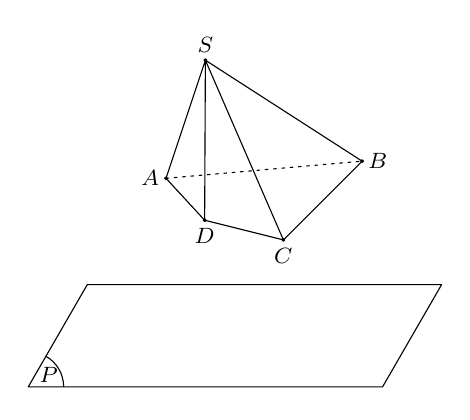
\begin{tikzpicture}[scale=0.5, >=stealth, line join=round, line cap=round, font=\footnotesize]
			\path
			(0,0) coordinate (A)
			++(5:5) coordinate (B)
			++(-2,-2) coordinate (C)
			++(-2,.5) coordinate (D) 
			(A)++(1,3) coordinate (S)
			;
			\draw [dash pattern=on 1pt off 2pt] (A)--(B);
			\draw (C)--(B) (D)--(C) (B)--(S) (C)--(S) (D)--(S)  (A)--(D) (A)--(S)
			(A)++(-2,-2.7)--++(0:9)--++(-120:3)--++(180:9)--cycle
			(A)++(-2,-2.7)++(-120:3)++(0:.9) arc (0:60:.9)
			(A)++(-2,-2.7)++(-120:3)++(30:.6) node {$P$}
			;
			\foreach \x/\y in {S/90,A/180,B/0,C/-90,D/-90}{
				\draw [fill=black] (\x) circle (1pt) ++(\y:0.4) node {$\x$};
			}
		\end{tikzpicture}
	}
	\loigiai{
		\immini{
			Gọi $A'$ là giao điểm của đường thẳng $SA$ với mặt phẳng $(P)$. \\
			Suy ra $A'$ là ảnh của hai điểm $S$ và $A$ qua phép chiếu song song trên mặt phẳng $(P)$ theo phương chiếu $SA$. \\
			Qua $B$, $C$, $D$ lần lượt kẻ các đường thẳng song song với $SA$, cắt mặt phẳng $(P)$ tại $B'$, $C'$, $D'$. \\
			Suy ra $B'$, $C'$, $D'$ lần lượt là ảnh của $B$, $C$, $D$ qua phép chiếu song song trên mặt phẳng $(P)$ theo phương chiếu $SA$. \\
			Vậy tứ giác $A'B'C'D'$ là hình chiếu của hình chóp $S.ABCD$ qua phép chiếu song song trên mặt phẳng $(P)$ theo phương chiếu $SA$.
		}
		{
			\begin{tikzpicture}[scale=0.5,>=stealth,line join=round,line cap=round,font=\scriptsize]
				\path
				(0,0) coordinate (A)
				++(5:5) coordinate (B)
				++(-2,-2) coordinate (C)
				++(-2,.5) coordinate (D) 
				(A)++(1,3) coordinate (S)
				\foreach \x/\y in {A/1,B/1.2,C/1,D/1.1}{
					(\x)++($\y*(A)-\y*(S)$) coordinate (\x')
				}
				;
				\draw [dash pattern=on 1pt off 2pt] (A)--(B) (A')--(B');
				\draw (C)--(B) (D)--(C) (B)--(S) (C)--(S) (D)--(S)  (A)--(D) (A)--(S)
				(A)++(-2,-2.7)--++(0:8)--++(-120:3)--++(180:8)--cycle
				(A)++(-2,-2.7)++(-120:3)++(0:.9) arc (0:60:.9)
				(A)++(-2,-2.7)++(-120:3)++(30:.6) node {$P$}
				(B')--(C')--(D')--(A')
				(A)--(A') (B)--(B') (C)--(C') (D)--(D')
				;
				\foreach \x/\y in {S/90,A/180,B/0,C/-45,D/-150,A'/180,B'/0,C'/-90,D'/-90}{
					\draw [fill=black] (\x) circle (1pt) ++(\y:0.4) node {$\x$};
				}
			\end{tikzpicture}
		}
	}
\end{vd}
\begin{vd}%[1H4H6-1]%[Dự án đề cương 3 khối NH24-25-Dot2-Trương Tường]
	Cho hình hộp $ABCD.A'B'C'D'$. Gọi $O$ và $O'$ lần lượt là tâm của các hình bình hành $ABCD$ và $A'B'C'D'$.
	\begin{listEX}[1]
		\item Xác định ảnh của đoạn thẳng $AB$ qua phép chiếu song song trên mặt phẳng $(A'B'C'D')$ theo phương chiếu $BB'$.
		\item Xác định ảnh của tứ giác $ABCD$ qua phép chiếu song song trên mặt phẳng $(A'B'C'D')$ theo phương chiếu $OO'$. 
		\item Xác định ảnh của tam giác $A'C'D'$ qua phép chiếu song song trên mặt phẳng $(ABCD)$ theo phương chiếu $A'B$.
	\end{listEX}
	\loigiai{
		\begin{center}
			\begin{tikzpicture}[scale=0.7, >=stealth, line join=round, line cap=round, font=\footnotesize]
				\path (0,0) coordinate (A)
				++(0:5) coordinate (B)
				++(-2,-1.5) coordinate (C)
				++($(A)-(B)$) coordinate (D)
				\foreach \x in {A,B,C,D}{
					(\x)++(1,3) coordinate (\x')
				}
				($(A)!.5!(C)$) coordinate (O)
				($(A')!.5!(C')$) coordinate (O')
				($(C)!-1!(D)$) coordinate (E)
				;
				\coordinate (G) at (intersection cs:first line={(B')--(B)}, second line={(C')--(E)});
				
				\fill [gray!50] (A')--(C')--(D')--cycle (B)--(C)--(E);
				\draw (D)--(C) (A')--(B')--(C')--(D')--cycle  (C)--(C') (D)--(D') (A')--(C') (B')--(D') (D)--(E)  (C')--(E) (D')--(C) (G)--(B');
				\draw [dash pattern=on 1pt off 2pt] (D)--(A)--(B) (A)--(A') (O)--(O') (A)--(C) (B)--(D) (A')--(B)(C)--(B)--(E) (B)--(G);
				\foreach \x/\y in {A/170,B/10,C/-90,D/-90,A'/90,B'/90,C'/90,D'/180,E/-90,O/-90,O'/90}{
					\draw [fill=black] (\x) circle (1pt) ++(\y:0.4) node {$\x$};
				}
			\end{tikzpicture}
		\end{center}
		\begin{listEX}[1]
			\item Phép chiếu song song trên mặt phẳng $(A'B'C'D')$ theo phương chiếu $BB'$ biến 
			\begin{itemize}
				\item Điểm $A$ thành điểm $A'$ 
				\item Điểm $B$ thành điểm $B'$
			\end{itemize}
			Vậy đoạn thẳng $A'B'$ là ảnh của đoạn thẳng $AB$ qua phép chiếu song song trên mặt phẳng $(A'B'C'D')$ theo phương chiếu $BB'$. 
			\item Phép chiếu song song trên mặt phẳng $(A'B'C'D')$ theo phương chiếu $OO'$ biến các điểm $A$, $B$, $C$, $D$ lần lượt thành các điểm $A'$, $B'$, $C'$, $D'$. \\
			Vậy tứ giác $A'B'C'D'$ là ảnh của tứ giác $ABCD$ qua phép chiếu song song trên mặt phẳng $(A'B'C'D')$ theo phương chiếu $OO'$. 
			\item Trong mặt phẳng $(CDD'C')$ dựng điểm $E$ sao cho $D'CEC'$ là hình bình hành. \\
			Khi đó ta có $A'B \parallel D'C \parallel C'E$. \\
			Phép chiếu song song trên mặt phẳng $(ABCD)$ theo phương chiếu $A'B$ biến các điểm $A'$, $C'$, $D'$ lần lượt thành các điểm $B$, $E$, $C$.\\
			Vậy tam giác $BEC$ là ảnh của tam giác $A'C'D'$ qua phép chiếu song song trên mặt phẳng $(ABCD)$ theo phương chiếu $A'B$.
		\end{listEX}
	}
\end{vd}
\begin{vd}%[1H4H6-5]%[Dự án đề cương 3 khối NH24-25-Dot2-Trương Tường]
	Cho hình lăng trụ $ABC.A'B'C'$. Gọi $M$, $N$ lần lượt là các điểm thuộc cạnh $AB$, $AC$ sao cho $\dfrac{AM}{AB} = \dfrac{AN}{AC} = \dfrac{1}{3}$; $P$, $Q$ lần lượt là tâm các mặt bên $ABB'A'$, $ACC'A'$. Hình chiếu song song của đoạn thẳng $MN$ và $PQ$ theo phương $AC$ lên mặt phẳng $(BB'C'C)$ lần lượt là là đoạn thẳng $M'N'$ và $P'Q'$. Tính tỉ số $\dfrac{M'N'}{P'Q'}$.
	\loigiai{
		\immini{
			Xét tam giác $ABC$ có $\dfrac{AM}{AB}=\dfrac{AN}{AC}=\dfrac{1}{3}$ nên theo định lí Thalès đảo ta có $MN \parallel BC$. \\
			Suy ra $\dfrac{MN}{BC}=\dfrac{AM}{AB}=\dfrac{1}{3}$ hay $MN=\dfrac{BC}{3}$. \\
			Xét tam giác $A'BC$ có $PQ$ là đường trung bình nên $PQ \parallel BC$ và $PQ=\dfrac{BC}{2}$. \\
			Ta có: $MN \parallel PQ$ (vì cùng song song $BC$) nên theo tính chất của phép chiếu song song ta có 
			$$\dfrac{M'N'}{P'Q'}=\dfrac{MN}{PQ}=\dfrac{\dfrac{BC}{3}}{\dfrac{BC}{2}}=\dfrac{2}{3}.$$
		}
		{
			\begin{tikzpicture}[scale=0.7, >=stealth, line join=round, line cap=round, font=\footnotesize]
				\path (0,0) coordinate (A)
				++(6,0) coordinate (B)
				++(-4.5,-1.5) coordinate (C)
				\foreach \x in {A,B,C}{
					(\x)++(.5,4) coordinate (\x')
				}
				($(A)!1/3!(B)$) coordinate (M)
				($(A)!1/3!(C)$) coordinate (N)
				($(A')!1/2!(B)$) coordinate (P)
				($(A')!1/2!(C)$) coordinate (Q)
				;
				\draw (A)--(C)--(B) (A')--(B')--(C')--cycle (A)--(A') (B)--(B') (C)--(C') (A')--(C) (A)--(C');
				\draw [dash pattern=on 1pt off 2pt] (A)--(B) (M)--(N) (A')--(B) (A)--(B') (P)--(Q);
				\foreach \x/\y in {A/180,B/0,C/-90,A'/90,B'/90,C'/-160,M/90,N/-135,P/0,Q/180}{
					\draw [fill=black] (\x) circle (1pt) ++(\y:0.4) node {$\x$};
				}
			\end{tikzpicture}
		}
	}
\end{vd}
%%%%%%%%%%%

\begin{dang}{Bài toán - Vẽ hình biểu diễn của hình không gian}
	\begin{itemize}
		\item Sử dụng các quy  tắc vẽ hình biểu diễn của hình không gian.
	\end{itemize}
\end{dang}
\begin{vd}%[1H4N6-2]%[Dự án đề cương 3 khối NH24-25-Dot2-Trương Tường]
	Vẽ hình biểu diễn của một hình lăng trụ tứ giác có đáy là hình thang với đáy lớn gấp $2$ lần đáy bé. 
	\loigiai{
		\immini{
			\begin{itemize}
				\item Hai đáy của hình lăng trụ là hình thang với đáy lớn gấp $2$ lần đáy bé nên hình biểu diễn cũng là hình thang có đáy lớn gấp $2$ lần đáy bé. 
				\item Các mặt bên của hình lăng trụ là hình bình hành nên được biểu diễn bằng hình bình hành.
			\end{itemize}
		}
		{
			\begin{tikzpicture}[scale=0.6, >=stealth, line join=round, line cap=round, font=\footnotesize]
				\path (0,0) coordinate (A)
				+(0:6) coordinate (B)
				+(1.5,-1.5) coordinate (D)
				(D)++($.5*(B)-.5*(A)$) coordinate (C)
				\foreach \x in {A,B,C,D}{
					(\x) ++(1,3) coordinate (\x')
				}
				;
				\draw (B)--(C)--(D)--(A) (A')--(B')--(C')--(D')--cycle (B)--(B') (C)--(C') (A)--(A') (D)--(D');
				\draw [dash pattern=on 1pt off 2pt] (A)--(B);
			\end{tikzpicture}
		}
	}
\end{vd}
\begin{vd}%[1H4H6-2]%[Dự án đề cương 3 khối NH24-25-Dot2-Trương Tường]
	Vẽ hình biểu diễn của một tam giác đều. 
	\loigiai{
		\begin{itemize}
			\item [\faCaretRight] Phân tích:
		\end{itemize}
		Gọi $O$ là tâm tam giác đều $ABC$, $D$ là điểm đối xứng với $A$ qua $O$. \\
		Khi đó:
		\immini{
			\begin{itemize}
				\item Tứ giác $BOCD$ là hình thoi. 
				\item $O$ là trung điểm của $AD$. 
			\end{itemize}
		}
		{
			\begin{tikzpicture}[scale=0.5, >=stealth, line join=round, line cap=round, font=\footnotesize]
				\def\a{6}
				\pgfmathsetmacro\r{\a*sqrt(3)/3}
				\path
				(0,0) coordinate (B) ++(0:\a) coordinate (C)
				($(B)!1!60:(C)$) coordinate (A) 
				($1/3*(A)+1/3*(B)+1/3*(C)$) coordinate (O)
				($(O)!-1!(A)$) coordinate (D)
				;
				\draw (A)--(B)--(C)--cycle (O) circle (\r) (C)--(D) (B)--(O)--(C)--(D)--cycle (A)--(D);
				\foreach \x/\y in {A/90,B/-135,C/-45,O/20,D/-90}{
					\draw [fill=black] (\x) circle (1pt) ++(\y:0.4) node {$\x$};
				}
			\end{tikzpicture}
		}
		\begin{itemize}
			\item [\faCaretRight] Vẽ:
		\end{itemize}
		\immini{
			\begin{itemize}
				\item Vẽ hình bình hành $B'O'C'D'$ biểu diễn hình thoi $BOCD$. 
				\item Gọi $A'$ đối xứng với $D'$ qua $O'$. 
			\end{itemize}
			Vậy tam giác $A'B'C'$ là hình biểu diến tam giác đều $ABC$.
		}
		{
			\begin{tikzpicture}[scale=0.5, >=stealth, line join=round, line cap=round, font=\footnotesize]
				\path
				(0,0) coordinate (B') 
				++(0:5) coordinate (D')
				++(60:3) coordinate (C')
				++($(B')-(D')$) coordinate (O')
				($(O')!-1!(D')$) coordinate (A')
				;
				\draw (A')--(B')--(C')--cycle (O') (C')--(D') (B')--(O')--(C')--(D')--cycle (A')--(D');
				\foreach \x/\y in {A'/90,B'/-135,C'/0,O'/60,D'/-90}{
					\draw [fill=black] (\x) circle (1pt) ++(\y:0.5) node {$\x$};
				}
			\end{tikzpicture}
		}
	}
\end{vd}
\begin{vd}%[1H4H6-2]%[Dự án đề cương 3 khối NH24-25-Dot2-Trương Tường]
	Vẽ hình biểu diễn của một đường tròn có hai đường kính vuông góc với nhau. 
	\loigiai{
		\begin{itemize}
			\item [\faCaretRight] Phân tích: \\
			Gỉả sử hình thực tế là đường tròn $(O)$ và hai đường kính $AB$ và $CD$ vuông góc với nhau. \\
			Khi đó:
		\end{itemize}
		\immini{
			\begin{itemize}
				\item Hình biểu diễn của đường tròn tâm $O$ là đường elip tâm $(O')$. 
				\item Hình biểu diễn của đường kính $AB$ là đoạn thẳng $A'B'$ qua tâm $O'$. 
				\item Gọi $MN$ là dây bất kí song song với $AB$ thì $MN$ cắt $CD$ tại trung điểm của $CD$. \\
				Như vậy, nếu hình biểu diễn của dây $MN$ là đoạn thẳng $M'N'$ thì $M'N'$ song song với $A'B'$.\\
				Hình biểu diễn của đường kính $CD$ là đoạn thẳng qua $O'$ và trung điểm của $M'N'$.   
			\end{itemize}
		}
		{
			\begin{tikzpicture}[scale=0.7, >=stealth, line join=round, line cap=round, font=\footnotesize]
				\def\r{2}
				\path
				(0,0) coordinate (O)
				+(180:\r) coordinate (A)
				+(0:\r) coordinate (B)
				+(90:\r) coordinate (C)
				+(-90:\r) coordinate (D)
				+(30:\r) coordinate (N)
				+(150:\r) coordinate (M)
				($(M)!.5!(N)$) coordinate (I)
				;
				\draw (A)--(B) (C)--(D) (O) circle (\r);
				\draw [dash pattern=on 1pt off 2pt] (M)--(N);
				\foreach \x/\y in {A/180,B/0,C/90,O/-45,D/-90,M/180,N/0,I/-45}{
					\draw [fill=black] (\x) circle (1pt) ++(\y:0.4) node {$\x$};
				}
				\pic [draw, angle radius=0.15cm, angle eccentricity=1.5] {right angle=B--O--C};
				\pic [draw, angle radius=0.15cm, angle eccentricity=1.5] {right angle=N--I--C};
			\end{tikzpicture}
		}
		\begin{itemize}
			\item [\faCaretRight] Vẽ:
		\end{itemize}
		\immini{
			\begin{itemize}
				\item Vẽ đường elip tâm $O'$ biểu diễn đường tròn tâm $O$. 
				\item Vẽ đoạn $A'B'$ qua tâm $O'$ biểu diễn đường kính $AB$.
				\item Vẽ đoạn $M'N'$ tùy ý song song với $A'B'$ và xác định trung điểm $I'$ của $M'N'$. 
				\item Vẽ đoạn thẳng $C'D'$ qua hai điểm $O'$ và $I'$ biểu diễn đường kính $CD$.  
			\end{itemize}
			Vậy elip tâm $O'$ cùng với hai đoạn thẳng $A'B'$ và $C'D'$ là hình biểu diến của đường tròn có hai đường kính vuông góc với nhau.
		}
		{
			\begin{tikzpicture}[scale=0.7, >=stealth, line join=round, line cap=round, font=\footnotesize]
				\def\a{3}
				\def\b{1}
				\path
				(0,0) coordinate (O')
				($({\a*cos(45)},{\b*sin(45)})+(O')$) coordinate (B')
				($({\a*cos(60)},{\b*sin(60)})+(O')$) coordinate (N')
				($({\a*cos(205)},{\b*sin(205)})+(O')$) coordinate (M')
				($(O')!-1!(B')$) coordinate (A')
				($(M')!.5!(N')$) coordinate (I')
				;
				\path [name path=d] (O')++($5*(I')-5*(O')$)--++($10*(O')-10*(I')$);
				\path [draw, name path=e] (O') ellipse ({\a} and {\b});
				\path [name intersections={of=d and e, by={C',D'}}];
				%
				\draw (A')--(B') (C')--(D');
				\draw [dash pattern=on 1pt off 2pt] (M')--(N');
				\foreach \x/\y in {A'/-135,B'/45,C'/90,O'/-90,D'/-90,M'/-135,N'/45,I'/90}{
					\draw [fill=black] (\x) circle (1pt) ++(\y:0.4) node {$\x$};
				}
				\pic [draw, angle radius=0.15cm, angle eccentricity=1.5] {right angle=B'--O'--C'};
				\pic [draw, angle radius=0.15cm, angle eccentricity=1.5] {right angle=N'--I'--C'};
			\end{tikzpicture}
		}
	}
\end{vd}
%-----------------------------------------------------------------------------
\subsection{Bài tập rèn luyện}
\ind{PHẦN I.} \inden{Câu trắc nghiệm nhiều phương án lựa chọn. Mỗi câu hỏi học sinh chỉ chọn một phương án.}\\
\setcounter{ex}{0}
\Opensolutionfile{ans}[ans/1H4-Bai5-TN]
\begin{ex}%[1H4N6-1]%[Dự án đề cương 3 khối NH24-25-Dot2-Trương Tường]
	Trong không gian cho mặt phẳng $(P)$ và đường thẳng $l$ cắt $(P)$ tại điểm $M$. Gọi $A$ là điểm tùy ý trên $l$ và gọi $A'$ là ảnh của $A$ qua phép chiếu song song trên $(P)$ theo phương chiếu $l$. Mệnh đề nào sau đây là đúng? 
	\choice
	{$AA'$ song song với $l$}
	{$A'$ trùng $A$}
	{\True $A'$ trùng $M$}
	{$AA'$ song song với $(P)$}
	\loigiai{
		Từ khái niệm phép chiếu song song ta có $A'$ trùng $M$. 
	}
\end{ex}
\begin{ex}%[1H4N6-1]%[Dự án đề cương 3 khối NH24-25-Dot2-Trương Tường]
	(\textit{Trích Đề cuối kỳ I Toán 11 năm 2024 – 2025 trường chuyên Lê Thánh Tông – Quảng Nam}) \\
	Cho hình chóp $S.ABCD$ có đáy $ABCD$ là hình bình hành. Hình chiếu song song của điểm $A$ theo phương $CD$ lên mặt phẳng $(SBC)$ là điểm nào sau đây?
	\choice
	{$S$}
	{$C$}
	{\True $B$}
	{$A$}
	\loigiai{
		Vì $AB \parallel CD$ và $AB$ cắt $(SBC)$ tại $B$ nên $B$ là hình chiếu song song của $A$ theo phương $CD$ lên mặt phẳng $(SBC)$.
	}
\end{ex}
\begin{ex}%[1H4N6-1]%[Dự án đề cương 3 khối NH24-25-Dot2-Trương Tường]
	(\textit{Trích Đề cuối kì I Toán 11 năm 2024 – 2025 trường THPT Chế Lan Viên – Quảng Trị}) \\
	Chọn khẳng định đúng trong các khẳng định sau
	\choice
	{Phép chiếu song song biến hai đường thẳng song song thành hai đường thẳng song song}
	{Phép chiếu song song biến hai đường thẳng song song thành hai đường thẳng trùng nhau}
	{\True Phép chiếu song song biến hai đường thẳng song song thành hai đường thẳng song song hoặc trùng nhau}
	{Phép chiếu song song biến hai đường thẳng song song thành hai đường thẳng chéo nhau}
	\loigiai{
		Theo tính chất phép chiếu song song ta có \\
		Phép chiếu song song biến hai đường thẳng song song thành hai đường thẳng song song hoặc trùng nhau.
	}
\end{ex}
\begin{ex}%[1H4N6-1]%[Dự án đề cương 3 khối NH24-25-Dot2-Trương Tường]
	(\textit{Trích Đề cuối kỳ I Toán 11 năm 2024 – 2025 trường THPT Lê Lợi – Quảng Trị}) \\
	Trong các mệnh đề sau mệnh đề nào sai?
	\choice
	{\True Phép chiếu song song biến hai đường thẳng song song thành hai đường thẳng song song}
	{Phép chiếu song song biến ba điểm thẳng hàng thành ba điểm thẳng hàng và không làm thay đổi thứ tự của ba điểm đó}
	{Phép chiếu song song biến đoạn thẳng thành đoạn thẳng}
	{Phép chiếu song song giữ nguyên tỉ số độ dài của hai đoạn thẳng cùng nằm trên một đường thẳng hoặc nằm trên hai đường thẳng song song}
	\loigiai{
		Theo tính chất phép chiếu song song ta có \\
		Phép chiếu song song biến hai đường thẳng song song thành hai đường thẳng song song hoặc trùng nhau.
	}
\end{ex}
\begin{ex}%[1H4N6-1]%[Dự án đề cương 3 khối NH24-25-Dot2-Trương Tường]
	Mệnh đề nào sau đây là sai?
	\choice
	{Phép chiếu song song biến ba điểm thẳng hàng thành ba điểm thẳng hàng}
	{Phép chiếu song song biến đoạn thẳng thành đoạn thẳng}
	{Phép chiếu song song giữ nguyên tỉ số giữa hai đoạn thẳng nằm trên cùng một đường thẳng}
	{\True Phép chiếu song song bảo toàn tỉ số giữa hai đoạn thẳng nằm trên hai đường thẳng chéo nhau}
	\loigiai{
		Theo tính chất phép chiếu song song ta có \\
		Phép chiếu song song \textbf{không} bảo toàn tỉ số giữa hai đoạn thẳng nằm trên hai đường thẳng chéo nhau.
	}
\end{ex}
\begin{ex}%[1H4N6-1]%[Dự án đề cương 3 khối NH24-25-Dot2-Trương Tường]
	(\textit{Trích Đề cuối kì I Toán 11 năm 2024 – 2025 trường chuyên Lê Khiết – Quảng Ngãi}) \\
	Qua phép chiếu song song trong không gian, hình chiếu của hình chữ nhật không thể là hình nào trong các hình sau?
	\choice
	{Hình vuông}
	{Hình bình hành}
	{Hình thoi}
	{\True Hình thang}
	\loigiai{
		Theo tính chất phép chiếu song song ta có \\
		Qua phép chiếu song song trong không gian, hình chiếu của hình chữ nhật không thể là hình thang.
	}
\end{ex}
\begin{ex}%[1H4N6-2]%[Dự án đề cương 3 khối NH24-25-Dot2-Trương Tường]
	(\textit{Trích Đề cuối học kì I Toán 11 năm 2024 – 2025 trường THPT Nguyễn Du – Bà Rịa Vũng Tàu}) \\
	Cho các hình vẽ dưới đây \\
	\centerline{
		\begin{tikzpicture}[scale=0.6, >=stealth, line join=round, line cap=round]
			\path (0,0) coordinate (A)
			++(0:4) coordinate (B)
			++(-1.5,-1.5) coordinate (C)
			++($(A)-(B)$) coordinate (D)
			\foreach \x in {A,B,C,D}{
				(\x)++(0,3) coordinate (\x')
			};
			\draw (D)--(C)--(B) (A')--(B')--(C')--(D')--cycle (B)--(B') (C)--(C') (D)--(D');
			\draw [dash pattern=on 1pt off 2pt] (D)--(A)--(B) (A)--(A');
			\draw ($(C)!.5!(D)$) node [below=.3cm]  {Hình 1};
		\end{tikzpicture}
		\hspace*{1cm}
		\begin{tikzpicture}[scale=0.6, >=stealth, line join=round, line cap=round]
			\path (0,0) coordinate (A)
			++(0:4) coordinate (B)
			++(-1.5,-1.5) coordinate (C)
			++(-1.5,.4) coordinate (D)
			\foreach \x in {A,B,C,D}{
				(\x)++(0,3) coordinate (\x')
			};
			\draw (A)--(D)--(C)--(B) (A')--(B')--(C')--(D')--cycle (B)--(B') (C)--(C') (D)--(D') (A)--(A');
			\draw [dash pattern=on 1pt off 2pt] (A)--(B);
			\draw ($(C)!.5!(D)$) node [below=.3cm]  {Hình 2};
		\end{tikzpicture}
		\hspace*{1cm}
		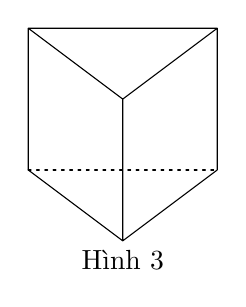
\begin{tikzpicture}[scale=0.6, >=stealth, line join=round, line cap=round]
			\path (0,0) coordinate (A)
			++(0:4) coordinate (B)
			++(-2,-1.5) coordinate (C)
			\foreach \x in {A,B,C}{
				(\x)++(0,3) coordinate (\x')
			};
			\draw (A)--(C)--(B) (A')--(B')--(C')--cycle (B)--(B') (C)--(C') (A)--(A');
			\draw [dash pattern=on 1pt off 2pt] (A)--(B);
			\draw (C) node [below]  {Hình 3};
		\end{tikzpicture}
		\hspace*{1cm}
		\begin{tikzpicture}[scale=0.6, >=stealth, line join=round, line cap=round]
			\path (0,0) coordinate (A)
			++(0:2) coordinate (B)
			++(2,-.5) coordinate (C)
			++(-1,-1) coordinate (D)
			++(-2,.25) coordinate (E)
			\foreach \x in {A,B,C,D,E}{
				(\x)++(0,3) coordinate (\x')
			};
			\draw (A)--(E)--(D)--(C) (A')--(B')--(C')--(D')--(E')--cycle (C)--(C') (D)--(D') (A)--(A') (E)--(E');
			\draw [dash pattern=on 1pt off 2pt] (A)--(B)--(C) (B)--(B');
			\draw ($(E)!.5!(D)$) node [below=.2cm]  {Hình 4};
		\end{tikzpicture}
	} \\ 
	Hình vẽ nào biểu diễn một hình lăng trụ ngũ giác?
	\choice 
	{Hình 1}
	{Hình 2}
	{Hình 3}
	{\True Hình 4}
	\loigiai{
		Hình 1 là hình biểu diễn của hình hộp. \\
		Hình 2 là hình biểu diễn của hình lăng trụ tứ giác. \\
		Hình 3 là hình biểu diễn của hình lăng trụ tam giác. \\
		Hình 4 là hình biểu diễn của một hình lăng trụ ngũ giác.
	}
\end{ex}
\begin{ex}%[1H4N6-4]%[Dự án đề cương 3 khối NH24-25-Dot2-Trương Tường]
	(\textit{Trích Đề cuối kì I Toán 11 năm 2024 – 2025 trường THPT Phan Bội Châu – Lâm Đồng})
	\immini{
		Chohình lập phương $ABCD.A'B'C'D'$. Điểm $B$ là hình chiếu của điểm $A$ trên mặt phẳng $(CBB'C')$ qua phép chiếu song song theo phương chiếu là đường thẳng nào? 
		\choice[1]
		{$BC$}
		{$CC'$}
		{$C'A'$}
		{\True $DC$}
	}
	{
		\begin{tikzpicture}[scale=0.6, >=stealth, line join=round, line cap=round, font=\footnotesize]
			\path (0,0) coordinate (A)
			++(0:3) coordinate (B)
			++(-1.5,-1.5) coordinate (C)
			++($(A)-(B)$) coordinate (D)
			\foreach \x in {A,B,C,D}{
				(\x)++(0,3) coordinate (\x')
			};
			\draw (D)--(C)--(B) (A')--(B')--(C')--(D')--cycle (B)--(B') (C)--(C') (D)--(D');
			\draw [dash pattern=on 1pt off 2pt] (D)--(A)--(B) (A)--(A');
			\foreach \x/\y in {A/180,B/0,C/-90,D/-90,A'/90,B'/90,C'/-30,D'/180}{
				\draw [fill=black] (\x) circle (1pt) ++(\y:0.4) node {$\x$};
			}
		\end{tikzpicture}
	}
	\loigiai{
		Vì điểm $B$ là hình chiếu của điểm $A$ qua một phép chiếu song song trên mặt phẳng $(CBB'C')$ và $BA \parallel DC$ nên phương chiếu là đường thẳng $DC$.
	}
\end{ex}
\begin{ex}%[1H4N6-1]%[Dự án đề cương 3 khối NH24-25-Dot2-Trương Tường]
	Trong không gian, cho đoạn thẳng $AB$ và gọi $A'B'$ là hình chiếu của của $AB$ qua một phép chiếu song song. Mệnh đề nào sau đây là đúng?
	\choice
	{Phép chiếu song song biến trung điểm của $AB$ thành điểm $A'$}
	{Phép chiếu song song biến trung điểm của $AB$ thành điểm $B'$}
	{\True Phép chiếu song song biến trung điểm của $AB$ thành trung điểm của $A'B'$}
	{Phép chiếu song song biến trung điểm của $AB$ thành điểm tùy ý trên $A'B'$}
	\loigiai{
		Giả sử phép chiếu song song biến $A$ thành $A'$ và $B$ thành $B'$ \\
		Gọi $M$ là trung điểm của $AB$ và $M'$ là ảnh của $M$ qua phép chiếu song song đã cho. \\
		Ta có $M'$ thuộc đoạn thẳng $A'B'$. \\
		Vì phép chiếu song song bảo toàn tỉ số hai đoạn thẳng cùng nằm trên một đường thẳng nên 
		$$\dfrac{MA}{MB}=\dfrac{M'A'}{M'B'}=1.$$
		Vậy $M'$ là trung điểm của đoạn thẳng $A'B'$.
	}
\end{ex}
\begin{ex}%[1H4N6-1]%[Dự án đề cương 3 khối NH24-25-Dot2-Trương Tường]
	Cho hình lăng trụ $ABC.A'B'C'$. Gọi $E$ là ảnh của điểm $C'$ qua phép chiếu song song trên mặt phẳng $(ABC)$ theo phương chiếu $A'B$. Khẳng định nào sau đây là \textbf{sai}? 
	\choice
	{$A'B \parallel C'E$}
	{$A'B=C'E$}
	{\True $E \in BC$}
	{$ABEC$ là hình bình hành}
	\loigiai{
		\immini{
			Vì $E$ là ảnh của điểm $C'$ qua phép chiếu song song trên mặt phẳng $(ABC)$ theo phương chiếu $A'B$ nên $A'C'EB$ là hình bình hành. \\
			Vậy $E$ không thuộc $BC$. 
		}
		{
			\begin{tikzpicture}[scale=0.7, >=stealth, line join=round, line cap=round, font=\footnotesize]
				\path (0,0) coordinate (A) 
				++(0:4) coordinate (C)
				++(-2.5,-1.5) coordinate (B)
				\foreach \x in {A,B,C}{
					(\x)++(1,3) coordinate (\x')
				}
				($(B)-(A')+(C')$) coordinate (E)
				;
				\draw (A)--(B) (A')--(B')--(C')--cycle
				(A)--(A') (B)--(B')  (C')--(E) (A')--(B)--(E)--(C');
				\draw [dash pattern=on 1pt off 2pt] (A)--(C) (C)--(E) (C)--(C') (B)--(C);
				\foreach \x/\y in {A/180,B/-90,C/0,A'/90,B'/90,C'/90,E/-90}{
					\draw [fill=black] (\x) circle (1pt) ++(\y:0.4) node {$\x$};
				}
			\end{tikzpicture}
		}
		
	}
\end{ex}
\begin{ex}%[1H4N6-1]%[Dự án đề cương 3 khối NH24-25-Dot2-Trương Tường]
	Cho hình lăng trụ tam giác $ABC.A'B'C'$. Gọi $O$ là điểm tùy ý thuộc miền trong tam giác $ABC$ và gọi điểm $O'$ là hình chiếu của $O$ trên mặt phẳng $(A'B'C')$ qua phép chiếu song song theo phương chiếu $AA'$. Mệnh đề nào sau đây là sai?
	\choice
	{$OO' \parallel AA'$}
	{$OO'=AA'$}
	{$OO' \parallel BB'$}
	{\True $OO' \subset (ABC)$}
	\loigiai{
		\immini{
			Điểm $O'$ là hình chiếu của $O$ trên mặt phẳng $(A'B'C')$ qua phép chiếu song song theo phương chiếu $AA'$ nên $OO' \parallel AA'$ nên $OO'$ \textbf{không thể} nằm trong mặt phẳng $(ABC)$.
		}
		{
			\begin{tikzpicture}[scale=0.7, >=stealth, line join=round, line cap=round, font=\footnotesize]
				\path (0,0) coordinate (A) 
				++(0:4) coordinate (C)
				++(-2.5,-1.5) coordinate (B)
				\foreach \x in {A,B,C}{
					(\x)++(-.5,3) coordinate (\x')
				}
				($1/3*(A)+1/3*(B)+1/3*(C)$) coordinate (O)
				++($(A')-(A)$) coordinate (O')
				;
				\draw (A)--(B)--(C) (A')--(B')--(C')--cycle
				(A)--(A') (B)--(B') (C)--(C')
				;
				\draw [dash pattern=on 1pt off 2pt] (A)--(C) (B')--(C') (O)--(O');
				\foreach \x/\y in {A/180,B/-90,C/0,A'/90,B'/80,C'/90,O/-90,O'/20}{
					\draw [fill=black] (\x) circle (1pt) ++(\y:0.4) node {$\x$};
				}
				\path ($(B)!0.5!(C)$) coordinate (M) ($(B')!0.5!(C')$) coordinate (M');
				\draw (A')--(M') ;
				\draw[dashed](A)--(M);
			\end{tikzpicture}			
		}
	}
\end{ex}

\begin{ex}%[1H4H6-1]%[Dự án đề cương 3 khối NH24-25-Dot2-Trương Tường]
	(\textit{Trích Đề cuối học kì I Toán 11 năm 2024 – 2025 trường THPT Kon Tum})
	\immini{
		Cho hình lăng trụ $ABC.A'B'C'$ (tham khảo hình vẽ bên).
		Phép chiếu song song lên mặt phẳng $(ABC)$ theo phương chiếu $A'A$ biến tam giác $AB'C'$ thành tam giác nào sau đây?
		\choice[1]
		{$A'B'C'$}
		{$AB'C'$}
		{\True $ABC$}
		{$A'BC$}
	}
	{
		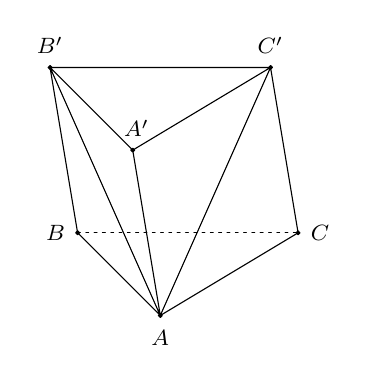
\begin{tikzpicture}[scale=0.7, >=stealth, line join=round, line cap=round, font=\footnotesize]
			\path (0,0) coordinate (B) 
			++(0:4) coordinate (C)
			++(-2.5,-1.5) coordinate (A)
			\foreach \x in {A,B,C}{
				(\x)++(-.5,3) coordinate (\x')
			}
			;
			\draw (B)--(A)--(C) (A')--(B')--(C')--cycle
			(A)--(A') (B)--(B') (C)--(C') (A)--(B') (C')--(A)--(B')
			;
			\draw [dash pattern=on 1pt off 2pt] (B)--(C);
			\foreach \x/\y in {B/180,A/-90,C/0,B'/90,A'/80,C'/90}{
				\draw [fill=black] (\x) circle (1pt) ++(\y:0.4) node {$\x$};
			}
		\end{tikzpicture}
	}
	\loigiai{
		Phép chiếu song song trên mặt phẳng $(ABC)$ theo phương $A'A$ biến điểm $A$ thành chính nó, biến điểm $B'$ và $C'$ theo thứ tự thành điểm $B$ và $C$, do đó sẽ biến tam giác $AB'C'$ thành tam giác $ABC$.
	}
\end{ex}
\begin{ex}%[1H4H6-2]%[Dự án đề cương 3 khối NH24-25-Dot2-Trương Tường]
	(\textit{Trích Câu 47 SBT 11 – Cánh Diều tập 11}) \\
	Trong các hình cho dưới đây, có bao nhiêu hình có thể là hình biểu diễn của một hình chóp tứ  giác? \\
	\centerline{
		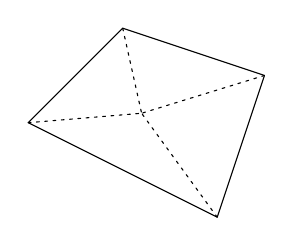
\begin{tikzpicture}[scale=1.2, >=stealth, line join=round, line cap=round, font=\footnotesize]
			\draw (0,0)--(1,1)--(2.5,.5)--(2,-1)--cycle;
			\draw [dash pattern=on 1pt off 2pt] (0,0)--(1.2,.1) (1,1)--(1.2,.1) (2.5,.5)--(1.2,.1) (2,-1)--(1.2,.1);
		\end{tikzpicture}
		\hspace*{3cm}
		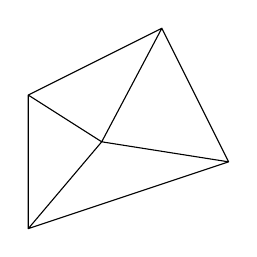
\begin{tikzpicture}[scale=1.2, >=stealth, line join=round, line cap=round, font=\footnotesize, rotate=45]
			\draw (0,0)--(1,1)--(2.5,.5)--(2,-1)--cycle
			(0,0)--(1.2,.1) (1,1)--(1.2,.1) (2.5,.5)--(1.2,.1) (2,-1)--(1.2,.1);
		\end{tikzpicture}
		\hspace*{3cm}
		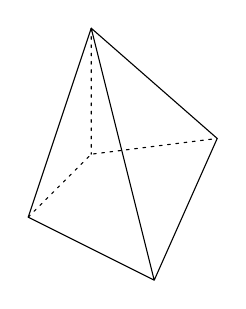
\begin{tikzpicture}[scale=.8, >=stealth, line join=round, line cap=round, font=\footnotesize]
			\draw (0,0)--(2,-1)--(3,1.25) (0,0)--(1,3) (2,-1)--(1,3) (1,3)--(3,1.25);
			\draw [dash pattern=on 1pt off 2pt] (0,0)--(1,1)--(3,1.25) (1,3)--(1,1);
		\end{tikzpicture}
	}
	\choice 
	{\True $3$}
	{$2$}
	{$1$}
	{$0$}
	\loigiai{
		Theo quy  tắc vẽ hình biểu diễn thì cả ba hình đều có thể là hình biểu diễn của một hình chóp tứ giác.
	}
\end{ex}
\begin{ex}%[1H4H6-1]%[Dự án đề cương 3 khối NH24-25-Dot2-Trương Tường]
	Cho hình hộp $ABCD.A'B'C'D'$. Tìm hình chiếu của đường thẳng $DD'$ qua phép chiếu song song trên mặt phẳng $(A'B'BA)$ theo phương chiếu $B'D'$? 
	\choice
	{\True Đường thẳng $BB'$}
	{Đường thẳng $CC'$}
	{Đường thẳng $AA'$}
	{Đường thẳng $A'B'$}
	\loigiai{
		\immini{
			Ta có điểm $B$ và $B'$ lần lượt là ảnh của điểm $D$ và $D'$ qua phép chiếu song song trên mặt phẳng $(A'B'BA)$ theo phương chiếu $B'D'$. \\
			Vậy đường thẳng $BB'$ là hình chiếu của đường thẳng $DD'$ qua phép chiếu song song trên mặt phẳng $(A'B'BA)$ theo phương chiếu $B'D'$.
		}
		{
			\begin{tikzpicture}[scale=0.6, >=stealth, line join=round, line cap=round, font=\footnotesize]
				\path (0,0) coordinate (A)
				++(0:4) coordinate (B)
				++(-1.5,-1.5) coordinate (C)
				++($(A)-(B)$) coordinate (D)
				\foreach \x in {A,B,C,D}{
					(\x)++(-1,3) coordinate (\x')
				}
				;
				\draw (D)--(C)--(B) (A')--(B')--(C')--(D')--cycle (B)--(B') (C)--(C') (D)--(D') (B')--(D');
				\draw [dash pattern=on 1pt off 2pt] (D)--(A)--(B) (A)--(A') (B)--(D);
				\foreach \x/\y in {A/170,B/10,C/-90,D/-90,A'/90,B'/90,C'/-10,D'/180}{
					\draw [fill=black] (\x) circle (1pt) ++(\y:0.4) node {$\x$};
				}
			\end{tikzpicture}
		}
	}
\end{ex}
\begin{ex}%[1H4H6-1]%[Dự án đề cương 3 khối NH24-25-Dot2-Trương Tường]
	(\textit{Trích Đề cuối kỳ I Toán 11 năm 2024 – 2025 trường THPT Phan Bội Châu – Khánh Hòa}) \\
	Cho hình chóp $S.ABCD$ có đáy $ABCD$ là hình bình hành tâm $O$. Hình chiếu song song của điểm $O$ lên $(SAD)$ theo phương của đường thẳng $SB$ là:
	\choice
	{Điểm $A$}
	{Điểm $D$}
	{Điểm $M$ là trung điểm của đoạn $SA$}
	{\True Điểm $N$ là trung điểm của đoạn $SD$}
	\loigiai{
		\immini{
			Xét tam giác $SBD$ có $ON$ là đường trung bình nên $ON \parallel SB$. \\
			Do đó $N$ là hình chiếu song song của điểm $O$ trên mặt phẳng $(SAD)$ theo phương chiếu $SB$.
		}
		{
			\begin{tikzpicture}[scale=0.7, >=stealth, line join=round, line cap=round, font=\footnotesize]
				\path (0,0) coordinate (A) 
				++(0:4) coordinate (B)
				++(-2,-1.5) coordinate (C)
				++($(A)-(B)$) coordinate (D)
				(A)++(1,3) coordinate (S)
				($(A)!.5!(C)$) coordinate (O)
				($(S)!.5!(B)$) coordinate (N)
				;
				\draw (D)--(C)--(B) (S)--(D) (S)--(C) (S)--(B);
				\draw [dash pattern=on 1pt off 2pt] (D)--(A)--(B) (S)--(A) (A)--(C) (B)--(D) (O)--(N);
				\foreach \x/\y in {A/180,B/0,C/-90,D/-90,S/90,O/-90,N/0}{
					\draw [fill=black] (\x) circle (1pt) ++(\y:0.4) node {$\x$};
				}
			\end{tikzpicture}
		}
	}
\end{ex}
\begin{ex}%[1H4H6-1]%[Dự án đề cương 3 khối NH24-25-Dot2-Trương Tường]
	(\textit{Trích Đề cuối kỳ I Toán 11 năm 2024 – 2025 trường THPT Nguyễn Quốc Trinh – Hà Nội})
	\immini{
		Cho hình chóp $S.ABCD$ có đáy là hình bình hành, gọi $M$ là trung điểm của cạnh $SC$ (tham khảo hình bên). Hình chiếu song song của điểm $M$ theo phương chiếu $AC$ trên mặt phẳng $(SAD)$ là điểm nào sau đây? 
		\choice[1]
		{Trung điểm của $SB$}
		{Trung điểm của $SD$}
		{\True Trung điểm của $SA$}
		{Điểm $D$}
	}
	{
		\begin{tikzpicture}[scale=0.7, >=stealth, line join=round, line cap=round, font=\footnotesize]
			\path (0,0) coordinate (A) 
			++(0:4) coordinate (B)
			++(-2,-1.5) coordinate (C)
			++($(A)-(B)$) coordinate (D)
			(A)++(1,3) coordinate (S)
			($(S)!.5!(C)$) coordinate (M)
			;
			\draw (D)--(C)--(B) (S)--(D) (S)--(C) (S)--(B);
			\draw [dash pattern=on 1pt off 2pt] (D)--(A)--(B) (S)--(A);
			\foreach \x/\y in {A/180,B/0,C/-90,D/-90,S/90,M/0}{
				\draw [fill=black] (\x) circle (1pt) ++(\y:0.4) node {$\x$};
			}
		\end{tikzpicture}
	}
	\loigiai{
		\immini{
			Gọi $N$ là trung điểm của $SA$. \\
			Xét tam giác $SAC$ có $MN$ là đường trung bình nên $MN \parallel AC$. \\
			Do đó $N$ là hình chiếu song song của điểm $M$ trên mặt phẳng $(SAD)$ theo phương chiếu $AC$.
		}
		{
			\begin{tikzpicture}[scale=0.7, >=stealth, line join=round, line cap=round, font=\footnotesize]
				\path (0,0) coordinate (A) 
				++(0:4) coordinate (B)
				++(-2,-1.5) coordinate (C)
				++($(A)-(B)$) coordinate (D)
				(A)++(1,3) coordinate (S)
				($(A)!.5!(S)$) coordinate (N)
				($(S)!.5!(C)$) coordinate (M)
				;
				\draw (D)--(C)--(B) (S)--(D) (S)--(C) (S)--(B);
				\draw [dash pattern=on 1pt off 2pt] (D)--(A)--(B) (S)--(A) (A)--(C) (B)--(D) (A)--(C) (M)--(N);
				\foreach \x/\y in {A/180,B/0,C/-90,D/-90,S/90,O/-90,N/0,M/0}{
					\draw [fill=black] (\x) circle (1pt) ++(\y:0.4) node {$\x$};
				}
			\end{tikzpicture}
		}
	}
\end{ex}
\begin{ex}%[1H4H6-1]%[Dự án đề cương 3 khối NH24-25-Dot2-Trương Tường]
	\immini{
		Cho hình hộp $ABCD.A'B'C'D'$. Tìm hình chiếu của đoạn thẳng $A'D'$ qua phép chiếu song song trên mặt phẳng $(ABCD)$ theo phương chiếu $CD'$?
		\choice[1]
		{\True Đoạn thẳng $BC$}
		{Đoạn thẳng $A'D'$}
		{Đoạn thẳng $AD$}
		{Đoạn thẳng $B'C'$}
	}
	{
		\begin{tikzpicture}[scale=0.6, >=stealth, line join=round, line cap=round, font=\footnotesize]
			\path (0,0) coordinate (A)
			++(0:4) coordinate (B)
			++(-1.5,-1.5) coordinate (C)
			++($(A)-(B)$) coordinate (D)
			\foreach \x in {A,B,C,D}{
				(\x)++(-1,4) coordinate (\x')
			}
			;
			\draw (D)--(C)--(B) (A')--(B')--(C')--(D')--cycle (B)--(B') (C)--(C') (D)--(D');
			\draw [dash pattern=on 1pt off 2pt] (D)--(A)--(B) (A)--(A');
			\foreach \x/\y in {A/170,B/10,C/-90,D/-90,A'/90,B'/90,C'/-10,D'/180}{
				\draw [fill=black] (\x) circle (1pt) ++(\y:0.4) node {$\x$};
			}
		\end{tikzpicture}
	}
	\loigiai{
		\immini{
			Ta có $CD' \parallel BA'$. \\
			Phép chiếu song song trên mặt phẳng $(ABCD)$ theo phương chiếu $CD'$ biến điểm $A'$ và $D'$ lần lượt thành điểm $B$ và $C$, do đó biến đoạn thẳng $A'D'$ thành đoạn thẳng $BC$.
		}
		{
			\begin{tikzpicture}[scale=0.6, >=stealth, line join=round, line cap=round, font=\footnotesize]
				\path (0,0) coordinate (A)
				++(0:4) coordinate (B)
				++(-1.5,-1.5) coordinate (C)
				++($(A)-(B)$) coordinate (D)
				\foreach \x in {A,B,C,D}{
					(\x)++(-.5,4) coordinate (\x')
				}
				;
				\draw (D)--(C)--(B) (A')--(B')--(C')--(D')--cycle (B)--(B') (C)--(C') (D)--(D') (C)--(D');
				\draw [dash pattern=on 1pt off 2pt] (D)--(A)--(B) (A)--(A') (B)--(A');
				\foreach \x/\y in {A/170,B/10,C/-90,D/-90,A'/90,B'/90,C'/-10,D'/180}{
					\draw [fill=black] (\x) circle (1pt) ++(\y:0.4) node {$\x$};
				}
			\end{tikzpicture}
		}
	}
\end{ex}
\begin{ex}%[1H4H6-1]%[Dự án đề cương 3 khối NH24-25-Dot2-Trương Tường]
	\immini{
		Cho hình hộp $ABCD.A'B'C'D'$. Gọi $M$, $N$ theo thứ tự là trung điểm của $A'B'$, $AC$ và đoạn thẳng $PQ$ là hình chiếu của đoạn thẳng $MN$ qua phép chiếu song song trên mặt phẳng $(CDD'C')$ theo phương chiếu $AD$. Khẳng định nào sau đây là \textbf{sai}?
		\choice[1]
		{$PQ \parallel AA'$}
		{$PQ=BB'$}
		{\True $MN \parallel PQ$}
		{$PQ \parallel (BCC'B')$}
	}
	{
		\begin{tikzpicture}[scale=0.6, >=stealth, line join=round, line cap=round, font=\footnotesize]
			\path (0,0) coordinate (A)
			++(0:4) coordinate (B)
			++(-1.5,-1.5) coordinate (C)
			++($(A)-(B)$) coordinate (D)
			\foreach \x in {A,B,C,D}{
				(\x)++(-.5,3) coordinate (\x')
			}
			($(A')!.5!(B')$) coordinate (M)
			($(A)!.5!(C)$) coordinate (N)
			;
			\draw (D)--(C)--(B) (A')--(B')--(C')--(D')--cycle (B)--(B') (C)--(C') (D)--(D');
			\draw [dash pattern=on 1pt off 2pt] (D)--(A)--(B) (A)--(A') (M)--(N) (A)--(C);
			\foreach \x/\y in {A/170,B/10,C/-90,D/-90,A'/90,B'/90,C'/-10,D'/180,M/90,N/10}{
				\draw [fill=black] (\x) circle (1pt) ++(\y:0.4) node {$\x$};
			}
		\end{tikzpicture}
	}
	\loigiai{
		\immini{
			Gọi $P$, $Q$ lần lượt là trung điểm của $C'D'$, $CD$. \\
			Khi đó $MP$ và $NQ$ song song với $AD$. \\
			Do đó $P$, $Q$ lần lượt là ảnh của $M$, $N$ trên mặt phẳng $CDD'C'$ theo phương chiếu $AD$. \\
			Như vậy $MN$ \textbf{không thể} song song với $PQ$. 
		}
		{
			\begin{tikzpicture}[scale=0.6, >=stealth, line join=round, line cap=round, font=\footnotesize]
				\path (0,0) coordinate (A)
				++(0:4) coordinate (B)
				++(-1.5,-1.5) coordinate (C)
				++($(A)-(B)$) coordinate (D)
				\foreach \x in {A,B,C,D}{
					(\x)++(-.5,3) coordinate (\x')
				}
				($(A')!.5!(B')$) coordinate (M)
				($(A)!.5!(C)$) coordinate (N)
				($(D')!.5!(C')$) coordinate (P)
				($(D)!.5!(C)$) coordinate (Q)
				;
				\draw (D)--(C)--(B) (A')--(B')--(C')--(D')--cycle (B)--(B') (C)--(C') (D)--(D') (P)--(Q) (M)--(P);
				\draw [dash pattern=on 1pt off 2pt] (D)--(A)--(B) (A)--(A') (M)--(N) (A)--(C) (N)--(Q);
				\foreach \x/\y in {A/170,B/10,C/-90,D/-90,A'/90,B'/90,C'/-10,D'/180,M/90,N/010,P/-45,Q/-90}{
					\draw [fill=black] (\x) circle (1pt) ++(\y:0.4) node {$\x$};
				}
			\end{tikzpicture}
		}
	}
\end{ex}
\begin{ex}%[1H4H6-1]%[Dự án đề cương 3 khối NH24-25-Dot2-Trương Tường]
	Cho tam giác $ABC$. Qua $A$, $B$, $C$ lần lượt dựng các đường thẳng $a$, $b$, $c$ song song với nhau và không nằm trong mặt phẳng $(ABC)$. Trên $a$, $b$, $c$ lần lượt lấy các điểm $A'$, $B'$, $C'$  tùy ý. Tìm hình chiếu song song của tam giác $A'B'C'$ trên mặt phẳng $(ABC)$ theo phương chiếu là đường thẳng $a$.
	\choice
	{Ba điểm $A$, $B$, $C$}
	{\True Tam giác $ABC$}
	{Tam giác $A'B'C'$}
	{Tam giác $AB'C'$}
	\loigiai{
		\immini{
			Ba điểm $A$, $B$, $C$ lần lượt là ảnh của ba điểm $A'$, $B'$, $C'$ trên mặt phẳng $(ABC)$ theo phương chiếu là đường thẳng $a$ nên tam giác $(ABC)$ là hình chiếu song song của tam giác $A'B'C'$ trên mặt phẳng $(ABC)$ theo phương chiếu là đường thẳng $a$.
		}
		{
			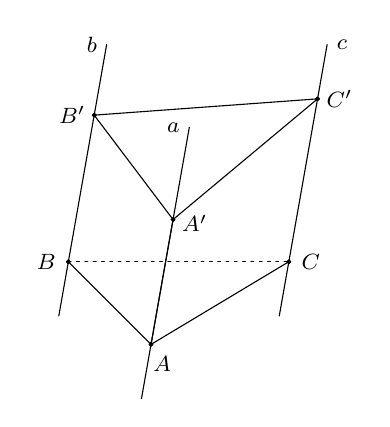
\begin{tikzpicture}[scale=0.7, >=stealth, line join=round, line cap=round, font=\footnotesize]
				\path (0,0) coordinate (B) 
				++(0:4) coordinate (C)
				++(-2.5,-1.5) coordinate (A)
				\foreach \x/\y in {A/2.3,B/2.7,C/3}{
					(\x)++(80:\y) coordinate (\x')
				}
				;
				\draw (B)--(A)--(C) (A')--(B')--(C')--cycle
				(A)--(A');
				\foreach \x/\y/\z in {A/a/{left},B/b/{left},C/c/{right}}{
					\draw (\x)++(-100:1)--++(80:5) node [\z] {$\y$};	
				}
				\draw [dash pattern=on 1pt off 2pt] (B)--(C);
				\foreach \x/\y in {B/180,A/-60,C/0,B'/180,A'/-10,C'/0}{
					\draw [fill=black] (\x) circle (1pt) ++(\y:0.4) node {$\x$};
				}
			\end{tikzpicture}
		}
	}
\end{ex}
\begin{ex}%[1H4H6-1]%[Dự án đề cương 3 khối NH24-25-Dot2-Trương Tường]
	\immini{
		Cho hình hộp $ABCD.A'B'C'D'$. Gọi đường thẳng $d$ là hình chiếu của đường thẳng $A'C$ trên mặt phẳng $(BDD'B')$ theo phương chiếu $AC$ (tham khảo hình bên). Mệnh đề nào sau đây là đúng? 
		\choice[1]
		{\True $d \parallel BB'$}
		{$d \parallel AC$}
		{$d \parallel BD$}
		{$d \parallel AB$}
	}
	{
		\begin{tikzpicture}[scale=0.6, >=stealth, line join=round, line cap=round, font=\footnotesize]
			\path (0,0) coordinate (A)
			++(0:4) coordinate (B)
			++(-1.5,-1.5) coordinate (C)
			++($(A)-(B)$) coordinate (D)
			\foreach \x in {A,B,C,D}{
				(\x)++(1,3) coordinate (\x')
			}
			;
			\fill [gray!50, opacity=.6] (D)--(D')--(B')--(B)--cycle;
			\draw (D)--(C)--(B) (A')--(B')--(C')--(D')--cycle (B)--(B') (C)--(C') (D)--(D')  (B')--(D');
			\draw [dash pattern=on 1pt off 2pt] (D)--(A)--(B) (A)--(A') (A)--(C) (B)--(D) (A')--(C) (A)--(C);
			\foreach \x/\y in {A/170,B/10,C/-90,D/-90,A'/90,B'/90,C'/-10,D'/180}{
				\draw [fill=black] (\x) circle (1pt) ++(\y:0.4) node {$\x$};
			}
		\end{tikzpicture}
	}
	\loigiai{
		\immini{
			Gọi $O$ và $O'$ theo thứ tự là tâm của hình bình hành $ABCD$ và $A'B'C'D'$. \\
			Suy ra $O'$ và $O$ theo thứ tự là ảnh của $A'$ và $C$ qua phép chiếu song song trên mặt phẳng $(BDD'B')$ theo phương chiếu $AC$. \\
			Do đó đường thẳng $OO'$ là hình chiếu của đường thẳng $A'C$ qua phép chiếu song song trên mặt phẳng $(BDD'B')$ theo phương chiếu $AC$. \\
			Như vậy đường thẳng $d$ trùng đường thẳng $OO'$. \\
			Nên $d \parallel BB'$.  
		}
		{
			\begin{tikzpicture}[scale=0.6, >=stealth, line join=round, line cap=round, font=\footnotesize]
				\path (0,0) coordinate (A)
				++(0:4) coordinate (B)
				++(-1.5,-1.5) coordinate (C)
				++($(A)-(B)$) coordinate (D)
				($(A)!.5!(C)$) coordinate (O)
				\foreach \x in {A,B,C,D,O}{
					(\x)++(1,3) coordinate (\x')
				}
				($(A)!.5!(C)$) coordinate (O)
				;
				\fill [gray!50, opacity=.6] (D)--(D')--(B')--(B)--cycle;
				\draw (D)--(C)--(B) (A')--(B')--(C')--(D')--cycle (B)--(B') (C)--(C') (D)--(D')  (B')--(D') (A')--(C');
				\draw [dash pattern=on 1pt off 2pt] (D)--(A)--(B) (A)--(A') (A)--(C) (B)--(D) (A')--(C) (A)--(C) (O)--(O');
				\foreach \x/\y in {A/170,B/10,C/-90,D/-90,A'/90,B'/90,C'/-10,D'/180,O/-90,O'/90}{
					\draw [fill=black] (\x) circle (1pt) ++(\y:0.4) node {$\x$};
				}
			\end{tikzpicture}
		}
	}
\end{ex}
\Closesolutionfile{ans}

\ind{PHẦN II.} \inden{Câu trắc nghiệm đúng sai. Trong mỗi ý a), b), c), d) ở mỗi câu, học sinh chọn đúng hoặc sai.}\\
\setcounter{ex}{0}
\Opensolutionfile{ans}[ans/2D1-Bai1-DS]%--Đặt tên 2D1-Bai1-DS
\begin{ex}%[1H4N6-2]%[Dự án đề cương 3 khối NH24-25-Dot2-Trương Tường]
	Xét phép chiếu song song mà hình phẳng không nằm trong mặt phẳng song song với phương chiếu. 
	\choiceTF
	{Hình biểu diễn của một tam giác đều là một tam giác đều}
	{Hình biểu diễn của một hình vuông là một hình thoi}
	{\True Hình biểu diễn của một hình tròn là hình elip} 
	{Hình biểu diễn của một hình thang cân là một hình thang cân}
	\loigiai{
		Theo tính chất của phép chiếu song song 
		\begin{itemchoice}
			\itemch Hình biểu diễn của một tam giác đều là một tam giác thường. 
			\itemch Hình biểu diễn của một hình vuông là một hình bình hành.
			\itemch Hình biểu diễn của một hình tròn là hình elip. 
			\itemch Hình biểu diễn của một hình thang cân là một hình thang.
		\end{itemchoice}
	}
\end{ex}
\begin{ex}%[1H4H6-1]%[Dự án đề cương 3 khối NH24-25-Dot2-Trương Tường]
	Cho hình hộp $ABCD.A'B'C'D'$. Gọi $O$ và $O'$ lần lượt là tâm các hình bình hành $ABCD$ và $A'B'C'D'$.
	\immini{
		\choiceTF
		{\True Nếu một phép chiếu song song biến điểm $C$ thành điểm $D$ thì phương chiếu song song với đường thẳng $CD$}
		{Nếu một phép chiếu song song biến tam giác $(ACD)$ thành tam giác $(A'C'D')$ thì mặt phẳng chiếu là $(ABCD)$}
		{\True Nếu phép chiếu song song trên mặt phẳng $(ABCD)$ theo phương chiếu $A'D$ biến điểm $O'$ thành điểm $I$ thì $A'O'ID$ là hình bình hành}
		{\True Phép chiếu song song trên mặt phẳng $(ACC'A')$ biến hình bình hành $BDD'B'$ thành đoạn thẳng $OO'$}
	}
	{
		\begin{tikzpicture}[scale=0.6, >=stealth, line join=round, line cap=round, font=\footnotesize]
			\path (0,0) coordinate (A)
			++(0:4) coordinate (B)
			++(-1.5,-1.5) coordinate (C)
			++($(A)-(B)$) coordinate (D)
			\foreach \x in {A,B,C,D}{
				(\x)++(-.5,3) coordinate (\x')
			}
			($(A)!.5!(C)$) coordinate (O)
			($(A')!.5!(C')$) coordinate (O')
			
			;
			\draw (D)--(C)--(B) (A')--(B')--(C')--(D')--cycle (B)--(B') (C)--(C') (D)--(D')  (B')--(D') (A')--(C');
			\draw [dash pattern=on 1pt off 2pt] (D)--(A)--(B) (A)--(A') (A)--(C) (B)--(D) (A)--(C);
			\foreach \x/\y in {A/170,B/10,C/-90,D/-90,A'/90,B'/90,C'/-10,D'/180,O/-90,O'/90}{
				\draw [fill=black] (\x) circle (1pt) ++(\y:0.4) node {$\x$};
			}
		\end{tikzpicture}
	}
	\loigiai{
		\centerline{
			\begin{tikzpicture}[scale=0.6, >=stealth, line join=round, line cap=round, font=\footnotesize]
				\path (0,0) coordinate (A)
				++(0:4) coordinate (B)
				++(-1.5,-1.5) coordinate (C)
				++($(A)-(B)$) coordinate (D)
				\foreach \x in {A,B,C,D}{
					(\x)++(-.5,3) coordinate (\x')
				}
				($(A)!.5!(C)$) coordinate (O)
				($(A')!.5!(C')$) coordinate (O')
				($(D)+(O')-(A')$) coordinate (I)
				($(D)!.5!(C')$) coordinate (K)
				($(D)!.5!(C)$) coordinate (J)
				($(D)!.5!(C')$) coordinate (F)
			;
			\draw (C)--(B) (I)--(J)--(C) (A')--(B')--(C')--(D')--cycle (B)--(B') (C)--(C') (D)--(D')  (B')--(D') (A')--(C') (D)--(I) (D)--(C') (F)--(I);
			\draw [dash pattern=on 1pt off 2pt] (D)--(A)--(B) (A)--(A') (A)--(C) (B)--(D) (A)--(C) (D)--(J) (O')--(F) (O)--(J);
				\draw [dash pattern=on 1pt off 2pt] (D)--(A)--(B) (A)--(A') (A)--(C) (B)--(D) (A)--(C) (O')--(K) (A')--(D) (O)--(O');
				\foreach \x/\y in {A/170,B/10,C/-90,D/-90,A'/90,B'/90,C'/-10,D'/180,O/-90,O'/90, I/-90}{
					\draw [fill=black] (\x) circle (1pt) ++(\y:0.4) node {$\x$};
				}
			\end{tikzpicture}
		} 
		\begin{itemchoice}
			\itemch Theo định nghĩa phép chiếu song ta có mệnh đề đúng. 
			\itemch Mặt phẳng chiếu chứa tam giác $A'C'D'$ nên phải là mặt phẳng $(A'B'C'D')$.
			\itemch Ta có $O'I \parallel A'D$. \\
			Vì $(A'B'C'D') \parallel (ABCD)$ nên $A'O' \parallel DI$. \\
			Vậy $A'O'ID$ là hình bình hành. 
			\itemch Phép chiếu song song trên mặt phẳng $(ACC'A')$ biến hai điểm $B$, $D$ thành điểm $O$, biến hai điểm $B'$, $D'$ thành điểm $O'$ nên biến hình bình hành $BDD'B'$ thành đoạn thẳng $OO'$. 
		\end{itemchoice}
	}
\end{ex}
\begin{ex}%[1H4H6-1]%[Dự án đề cương 3 khối NH24-25-Dot2-Trương Tường]
	Cho tam giác $ABC$. Xét tất cả các phép chiếu song song có phương chiếu không song song và không nằm trong mặt phẳng $(ABC)$; biến các đỉnh $A$, $B$, $C$ lần lượt thành các điểm $A'$, $B'$, $C'$.   
	\choiceTF
	{Mặt phẳng $(ABC)$ là mặt phẳng chiếu}
	{\True Các phép chiếu song song biến trung điểm cạnh $AB$ thành trung điểm cạnh $A'B'$}
	{\True Các phép chiếu song song biến trọng tâm tam giác $ABC$ thành trọng tâm tam giác $A'B'C'$}
	{$\triangle ABC$ đồng dạng với $\triangle A'B'C'$}
	\loigiai{
		\centerline{
			\begin{tikzpicture}[scale=0.7, >=stealth, line join=round, line cap=round, font=\footnotesize]
				\path (0,0) coordinate (B) 
				++(0:4) coordinate (C)
				++(-1.5,-1.5) coordinate (A)
				\foreach \x/\y in {A/2.3,B/2.7,C/3}{
					(\x)++(80:\y) coordinate (\x')
				}
				($(A)!.5!(B)$) coordinate (M)
				($(A')!.5!(B')$) coordinate (M')
				($(C)!2/3!(M)$) coordinate (G)
				($(C')!2/3!(M')$) coordinate (G')
				;
				\draw (B)--(A)--(C) (A')--(B')--(C')--cycle
				(A)--(A') (B)--(B') (C)--(C') (C')--(M') (M)--(M');
				\draw [dash pattern=on 1pt off 2pt] (B)--(C) (C)--(M) (G)--(G');
				\foreach \x/\y in {B/180,A/-80,C/0,B'/180,A'/-10,C'/0,M/-135,M'/-160,G/-90,G'/90}{
					\draw [fill=black] (\x) circle (1pt) ++(\y:0.4) node {$\x$};
				}
			\end{tikzpicture}
		} 
		Gọi $f$ là phép chiếu song song thỏa mãn đề bài. 
		\begin{itemchoice}
			\itemch Vị phép chiếu song song $f$ biến các đỉnh $A$, $B$, $C$ của tam giác $ABC$ lần lượt thành các điểm $A'$, $B'$, $C'$ nên mặt phẳng $(A'B'C')$ là mặt phẳng chiếu.
			\itemch Gọi $M$ là trung điểm của $AB$, $M'$ là ảnh của $M$ qua phép chiếu song song $f$. \\
			Theo tính chất phép chiếu song song ta có: $\dfrac{MA}{MB}=\dfrac{M'A'}{M'B'}=1$. \\
			Vậy $M'$ là  trung điểm của $A'B'$. 
			\itemch Gọi $G$ là trọng tâm tam giác $ABC$, $G'$ là ảnh của $G$ qua phép chiếu song song $f$. \\
			Khi đó, phép chiếu song song $f$ biến ba điểm thẳng hàng $A$, $G$, $M$ theo thứ tự thành ba điểm thẳng hàng $A'$, $G'$, $M'$ và đồng thời 
			$$\dfrac{CG}{CM}=\dfrac{C'G'}{C'M'}=\dfrac{2}{3}.$$
			Vậy $G'$ là trọng tâm của tam giác $A'B'C'$.
			\itemch Phép chiếu song song chỉ bảo toàn tỉ số hai đoạn thẳng cùng nằm trên một đường thẳng hoặc nằm trên hai đường thẳng song song nên trong trường hợp đề bài cho thì tỉ số $\dfrac{AB}{AC}$ không nhất thiết bằng tỉ số $\dfrac{A'B'}{A'C'}$.
		\end{itemchoice}
	}
\end{ex}
\begin{ex}%[1H4H6-1]%[Dự án đề cương 3 khối NH24-25-Dot2-Trương Tường]
	\immini{
		Cho hình lăng trụ tam giác $ABC.A'B'C'$. Gọi $E$, $F$ theo thứ tự là trung điểm của $A'B'$ và $A'C'$. 
		\choiceTF
		{\True Điểm $A'$ là ảnh của điểm $A$ qua phép chiếu song song trên mặt phẳng $(A'B'C')$ theo phương chiếu $BB'$}
		{Đoạn thẳng $AF$ là hình chiếu của đoạn thẳng $BE$ qua phép chiếu song song trên mặt phẳng $(ACC'A')$ theo phương chiếu $BC$}
		{\True Tam giác $ABC$ là hình chiếu của tam giác $C'AB$ qua phép chiếu song song trên mặt phẳng $(ABC)$ theo phương chiếu $AA'$}
		{\True Đường thẳng $BC$ là hình chiếu của đường thẳng $EF$ qua phép chiếu song song trên mặt phẳng $(ABC)$ theo phương chiếu $CF$}
	}
	{
		\begin{tikzpicture}[scale=0.7, >=stealth, line join=round, line cap=round, font=\footnotesize]
			\path (0,0) coordinate (A) 
			++(0:4) coordinate (B)
			++(-2.5,-1.5) coordinate (C)
			\foreach \x in {A,B,C}{
				(\x)++(.5,3) coordinate (\x')
			}
			($(A')!.5!(B')$) coordinate (E)
			($(A')!.5!(C')$) coordinate (F)
			;
			\draw (A)--(C)--(B) (A')--(B')--(C')--cycle
			(A)--(A') (B)--(B') (C)--(C')
			;
			\draw [dash pattern=on 1pt off 2pt] (A)--(B) (B')--(C');
			\foreach \x/\y in {A/180,B/0,C/-90,A'/90,B'/90,C'/80,E/90,F/-130}{
				\draw [fill=black] (\x) circle (1pt) ++(\y:0.4) node {$\x$};
			}
		\end{tikzpicture}
	}
	\loigiai{
		\centerline{
			\begin{tikzpicture}[scale=0.7, >=stealth, line join=round, line cap=round, font=\footnotesize]
				\path (0,0) coordinate (A) 
				++(0:4) coordinate (B)
				++(-2.5,-1.5) coordinate (C)
				\foreach \x in {A,B,C}{
					(\x)++(.5,3) coordinate (\x')
				}
				($(A')!.5!(B')$) coordinate (E)
				($(A')!.5!(C')$) coordinate (F)
				($(B)!.5!(C)$) coordinate (M)
				;
				\draw (A)--(C)--(B) (A')--(B')--(C')--cycle
				(A)--(A') (B)--(B') (C)--(C') (C)--(F) (E)--(F)
				;
				\draw [dash pattern=on 1pt off 2pt] (A)--(B) (B')--(C') (E)--(M) (B)--(E);
				\foreach \x/\y in {A/180,B/0,C/-90,A'/90,B'/90,C'/80,E/90,F/-130,M/-45}{
					\draw [fill=black] (\x) circle (1pt) ++(\y:0.4) node {$\x$};
				}
			\end{tikzpicture}
		}
		\begin{itemchoice}
			\itemch Vì $AA' \parallel BB'$ nên điểm $A'$ là ảnh của điểm $A$ qua phép chiếu song song trên mặt phẳng $(A'B'C')$ theo phương chiếu $BB'$. 
			\itemch Ta có $EF \parallel B'C' \parallel BC$ nên phép chiếu song song trên mặt phẳng $(ACC'A')$ biến các điểm $B$, $E$ theo thứ tự thành các điểm $C$, $F$. \\
			Vậy đoạn thẳng $CF$ là hình chiếu của đoạn thẳng $BE$ qua phép chiếu song song trên mặt phẳng $(ACC'A')$ theo phương chiếu $BC$.
			\itemch Phép chiếu song song trên mặt phẳng $(ABC)$ theo phương chiếu $AA'$ biến các điểm $A$, $B$, $C'$ lần lượt thành các điểm $A$, $B$, $C$. \\
			Vậy tam giác $ABC$ là hình chiếu của tam giác $C'AB$ qua phép chiếu song song trên mặt phẳng $(ABC)$ theo phương chiếu $AA'$.
			\itemch Gọi $M$ là trung điểm của $BC$. \\
			Ta có $EF \parallel CM$ và $EF=CM\left(=\dfrac{BC}{2}=\dfrac{B'C'}{2}\right)$. \\
			Suy ra $EFCM$ là hình bình hành. \\
			Nên $CF \parallel ME$. \\
			Do đó phép chiếu song song trên mặt phẳng $(ABC)$ theo phương chiếu $CF$ biến các điểm $E$, $F$ lần lượt thành các điểm $M$, $C$. \\
			Vậy đường thẳng $CM$ (cũng là đường thẳng $BC$) là hình chiếu của đường thẳng $EF$ qua phép chiếu song song trên mặt phẳng $(ABC)$ theo phương chiếu $CF$.
		\end{itemchoice}
	}
\end{ex}
\begin{ex}%[1H4V6-5]%[Dự án đề cương 3 khối NH24-25-Dot2-Trương Tường]
	Cho hình lăng trụ $ABCD.A'B'C'D'$ có đáy $ABCD$ là hình thang với $AB \parallel CD$ và $AB=2CD$. Gọi $M$ là điểm tùy ý trên cạnh $A'B'$. 
	\immini{
		\choiceTF
		{\True Điểm $A'$ là ảnh của điểm $A$ trên mặt phẳng $(A'B'C'D')$ qua phép chiếu song song theo phương chiếu $BB'$}
		{\True Đoạn thẳng $AD$ là hình chiếu của đoạn thẳng $A'D'$ trên mặt phẳng $(ABCD)$ qua phép chiếu song song theo phương chiếu $BB'$}
		{\True Đường thẳng $CD$ là hình chiếu của đường thẳng $A'B'$ trên mặt phẳng $(ABCD)$ qua phép chiếu song song theo phương chiếu $A'D$}
		{\True Hình chiếu của tam giác $MCD$ trên mặt phẳng $(ABCD)$ qua phép chiếu song song theo phương chiếu $BB'$ là một tam giác có diện tích bằng $\dfrac{1}{3}$ lần diện tích hình thang $ABCD$}
	}
	{
		\begin{tikzpicture}[scale=0.7, >=stealth, line join=round, line cap=round, font=\footnotesize]
			\path (0,0) coordinate (A)
			+(0:6) coordinate (B)
			+(1.5,-1.5) coordinate (D)
			(D)++($.5*(B)-.5*(A)$) coordinate (C)
			\foreach \x in {A,B,C,D}{
				(\x) ++(1,3) coordinate (\x')
			}
			;
			\draw (B)--(C)--(D)--(A) (A')--(B')--(C')--(D')--cycle (B)--(B') (C)--(C') (A)--(A') (D)--(D');
			\draw [dash pattern=on 1pt off 2pt] (A)--(B);
			\foreach \x/\y in {A/180,B/0,C/-90,D/-90,A'/90,B'/90,C'/-10,D'/180}{
				\draw [fill=black] (\x) circle (1pt) ++(\y:0.4) node {$\x$};
			}
		\end{tikzpicture}
	}
	\loigiai{
		\centerline{
			\begin{tikzpicture}[scale=0.7, >=stealth, line join=round, line cap=round, font=\footnotesize]
				\path (0,0) coordinate (A)
				+(0:6) coordinate (B)
				+(1.5,-1.5) coordinate (D)
				(D)++($.5*(B)-.5*(A)$) coordinate (C)
				\foreach \x in {A,B,C,D}{
					(\x) ++(1,3) coordinate (\x')
				}
				($(A')!.65!(B')$) coordinate (M)
				($(A)!.65!(B)$) coordinate (N)
				($(C)!-1!(D)$) coordinate (I)
				;
				\fill [black!40] (N)--(C)--(D)--cycle;
				\draw (C)--(D)--(A) (A')--(B')--(C')--(D')--cycle (C)--(C') (A)--(A') (D)--(D') (C)--(I) (A')--(D) (B')--(I);
				\draw [dash pattern=on 1pt off 2pt] (A)--(B) (C)--(N)--(D) (M)--(N) (B)--(B') (B)--(C) ;
				\foreach \x/\y in {A/180,B/0,C/-90,D/-90,A'/90,B'/90,C'/-10,D'/180,I/-90,M/90,N/110}{
					\draw [fill=black] (\x) circle (1pt) ++(\y:0.4) node {$\x$};
				}
			\end{tikzpicture}
		}
		\begin{itemchoice}
			\itemch Vì $AA' \parallel BB'$ và điểm $A'$ thuộc mặt phẳng $(A'B'C'D')$ nên điểm $A'$ là ảnh của điểm $A$ trên mặt phẳng $(A'B'C'D')$ qua phép chiếu song song theo phương chiếu $BB'$. 
			\itemch Hai điểm $A$ và $D$ lần lượt là ảnh của hai điểm $A'$ và $D'$ trên mặt phẳng $(ABCD)$ qua phép chiếu song song theo phương chiếu $BB'$. \\
			Vậy đoạn thẳng $AD$ là hình chiếu của đoạn thẳng $A'D'$ trên mặt phẳng $(ABCD)$ qua phép chiếu song song theo phương chiếu $BB'$.
			\itemch Gọi $I$ là điểm sao cho $C$ là trung điểm của $DI$. \\
			Tứ giác $A'B'ID$ có:
			\begin{itemize}
				\item $A'B'\parallel DI$.
				\item $A'B'=DI(=2CD)$.
			\end{itemize}
			Do đó $A'B'ID$ là hình bình hành. \\
			Như vậy đường thẳng $DI$ (cũng là đường thẳng $CD$) là hình chiếu của đường thẳng $A'B'$ trên mặt phẳng $ABCD$ qua phép chiếu song song theo phương chiếu $A'D$. 
			\itemch Gọi điểm $N$ là ảnh của điểm $M$ trên mặt phẳng $(ABCD)$ qua phép chiếu song song theo phương chiếu $BB'$. \\
			Khi đó $N$ thuộc đoạn thẳng $AB$.  \\
			Tam giác $NCD$ là hình chiếu của tam giác $MCD$ trên mặt phẳng $(ABCD)$ theo phương chiếu $BB'$. \\
			Gọi $h$ là chiều cao hình thang $ABCD$ ($h$ cũng là  chiều cao tam giác $MCD$).  \\
			Ta có $$\dfrac{S_{\triangle NCD}}{S_{ABCD}}=\dfrac{\dfrac{1}{2} \cdot CD \cdot h}{\dfrac{1}{2} \cdot (CD+AB) \cdot h}=\dfrac{CD}{3 \cdot CD}=\dfrac{1}{3}.$$
		\end{itemchoice}
	}
\end{ex}
\Closesolutionfile{ans}
%-------------------------------------------------------%
\ind{PHẦN III.} \inden{Câu trắc nghiệm Trả lời ngắn.} \\
\setcounter{ex}{0}
\Opensolutionfile{ans}[ans/1H4-Bai5-TLN]
\begin{ex}%[1H4V6-5]%[Dự án đề cương 3 khối NH24-25-Dot2-Trương Tường]
	(\textit{Trích Đề cuối kì I Toán 11 năm 2024 – 2025 trường THPT Phan Bội Châu – Lâm Đồng}) \\
	Cho tứ diện $ABCD$, $M$ là trọng tâm của tam giác $ABC$, $E$ là trung điểm của đoạn thẳng $AB$. Gọi $N$ là hình chiếu song song của điểm $M$ theo phương $CD$ lên mặt phẳng $(ABD)$. Khi đó tỉ số $\dfrac{EN}{ED}$ bằng bao nhiêu? (kết quả làm tròn đến hàng phần trăm).
	\shortans[oly]{$0,33$}
	\loigiai{
		\centerline{
			\begin{tikzpicture}[scale=0.7, >=stealth, line join=round, line cap=round, font=\footnotesize]
				\path 
				(0,0) coordinate (A)
				++(0:5) coordinate (B)
				++(-3,-2) coordinate (C)
				(A)+(1,3) coordinate (D)
				($1/3*(A)+1/3*(B)+1/3*(C)$) coordinate (M)
				($(A)!.5!(B)$) coordinate (E)
				($1/3*(A)+1/3*(B)+1/3*(D)$) coordinate (N)
				;
				\draw (A)--(C)--(B) (D)--(A) (D)--(B) (D)--(C);
				\draw [dash pattern=on 1pt off 2pt] (A)--(B) (C)--(E)--(D) (M)--(N);
				\foreach \x/\y in {A/180,B/0,C/-90,D/90,M/-45,E/45,N/45}{
					\draw [fill=black] (\x) circle (1pt) ++(\y:0.4) node {$\x$};
				}
			\end{tikzpicture}
		} \\
		Trong tam giác $CDE$, kẻ đường thẳng qua $M$, song song với $CD$, cắt $DE$ tại $N$. \\
		Suy ra $N$ là  hình chiếu song song của điểm $M$ trên mặt phẳng $(ABD)$ theo phương chiếu $CD$. \\
		Áp dụng định lí Thalès trong  tam giác $CDE$ ta có 
		$$\dfrac{EN}{ED}=\dfrac{EM}{EC}=\dfrac{1}{3} \approx 0{,}33.$$
	}
\end{ex}
\begin{ex}%[1H4V6-5]%[Dự án đề cương 3 khối NH24-25-Dot2-Trương Tường]
	Cho hình hộp $ABCD.A'B'C'D'$. Gọi $G$ và $G'$ theo thứ tự là trọng tâm tam giác $ACD$ và $ABC$; $O$ và $O'$ theo thứ tự là tâm các mặt bên $ADD'A'$ và $ABB'A'$. Tính tỉ số độ dài giữa hình chiếu của các đoạn thẳng $GG'$ và $OO'$ qua phép chiếu song song trên  mặt phẳng $(BCC'B')$ theo phương chiếu $DC$. Viết kết quả làm tròn đến hàng phần trăm.
	\shortans[oly]{$0,67$}
	\loigiai{
		\centerline{
			\begin{tikzpicture}[scale=0.6, >=stealth, line join=round, line cap=round, font=\footnotesize]
				\path (0,0) coordinate (A)
				++(0:5) coordinate (B)
				++(-1,-1.5) coordinate (C)
				++($(A)-(B)$) coordinate (D)
				\foreach \x in {A,B,C,D}{
					(\x)++(-1,4) coordinate (\x')
				}
				($(A)!.5!(D')$) coordinate (O)
				($(A)!.5!(B')$) coordinate (O')
				($(A)!.5!(C)$) coordinate (I)
				($1/3*(A)+1/3*(C)+1/3*(D)$) coordinate (G)
				($1/3*(A)+1/3*(B)+1/3*(C)$) coordinate (G')
				;
				\draw (D)--(C)--(B) (A')--(B')--(C')--(D')--cycle (B)--(B') (C)--(C') (D)--(D');
				\draw [dash pattern=on 1pt off 2pt] (D)--(A)--(B) (A)--(A') (A)--(C) (B)--(D) (A)--(C) (O)--(O') (G)--(G') (A')--(B) (A)--(B') (A)--(D') (A')--(D);
				\foreach \x/\y in {A/170,B/10,C/-90,D/-90,A'/90,B'/90,C'/-10,D'/180,O/180,O'/-90,G/-90,G'/-90,I/-90}{
					\draw [fill=black] (\x) circle (1pt) ++(\y:0.4) node {$\x$};
				}
			\end{tikzpicture}
		} \\
		Tam giác $A'BD$ có $O$ và $O'$ lần lượt là trung điểm của cạnh $A'D$ và $A'B$ nên $OO'$ là đường trung bình của tam giác $A'BD$. \\
		Suy ra $OO' \parallel BD$ và $OO'=\dfrac{1}{2}BD$. \\
		Vì $G$ và $G'$ theo thứ tự là trọng tâm tam giác $ACD$ và $ABC$ nên $G$ và $G'$ thuộc đoạn $BD$. \\
		Suy ra $GG' \parallel OO'$. \\
		Do đó tỉ số độ dài giữa hình chiếu của các đoạn thẳng $GG'$ và $OO'$ qua phép chiếu song song trên mặt phẳng $(BCC'B')$ bằng tỉ số $\dfrac{GG'}{OO'}$.
		Gọi $I$ là trung điểm $BD$. \\
		Theo tính chất trọng tâm tam giác ta có:
		$$GI=\dfrac{1}{3}DI=\dfrac{1}{6}BD \quad \text{và} \quad G'I=\dfrac{1}{3}BI=\dfrac{1}{6}BD.$$ 
		Do đó $GG'=GI+G'I=\dfrac{1}{3}BD$. \\
		Vậy $\dfrac{GG'}{OO'}=\dfrac{\dfrac{1}{3}BD}{\dfrac{1}{2}BD}=\dfrac{2}{3} \approx 0{,}67$.
	}
\end{ex}
\begin{ex}%[1H4V6-5]%[Dự án đề cương 3 khối NH24-25-Dot2-Trương Tường]
	Cho hình chóp $S.ABCD$. Gọi $G$ là trọng tâm tam giác $SAC$; $E$ là ảnh của điểm $G$ qua phép chiếu song song trên mặt phẳng $(SAD)$ theo phương chiếu $CD$. Đường thẳng $AE$ cắt cạnh $SD$ tại $F$. Tính tỉ số $\dfrac{EF}{EA}$. Viết kết quả làm tròn đến hàng phần chục.
	\shortans[oly]{$0,5$}   
	\loigiai{
		\centerline{
			\begin{tikzpicture}[scale=0.7, >=stealth, line join=round, line cap=round, font=\footnotesize]
				\path
				(0,0) coordinate (A)
				++(0:5) coordinate (B)
				++(-.75,-1.5) coordinate (C)
				++(-2.75,-.5) coordinate (D)
				(A)+(1,3) coordinate (S) 
				($1/3*(S)+1/3*(A)+1/3*(C)$) coordinate (G)
				($(A)!.5!(C)$) coordinate (O)
				($(A)!.5!(D)$) coordinate (M)
				($(S)!2/3!(M)$) coordinate (E)
				($(S)!.5!(D)$) coordinate (F)
				;
				\draw [dash pattern=on 1pt off 2pt] (A)--(B) (A)--(C) (S)--(O) (G)--(E) (O)--(M);
				\draw (C)--(B) (D)--(C) (B)--(S) (C)--(S) (D)--(S) (A)--(D) (A)--(S) (S)--(M) (A)--(F);
				\foreach \x/\y in {A/180,B/0,C/-90,D/-90,S/90,G/0,O/-90,M/-135,E/135,F/45}{
					\draw [fill=black] (\x) circle (1pt) ++(\y:0.3) node {$\x$};
				}
			\end{tikzpicture}
		} \\
		Gọi $O$ và $M$ lần lượt là trung điểm của $AC$ và $AD$. \\
		$OM$ là đường trung bình của tam giác $ACD$. \\
		Suy ra $OM \parallel CD$. \\
		Trong tam giác $SOM$, kẻ đường thẳng qua $G$, song song với $OM$ và cắt $SM$ tại $E$. \\
		$E$ là ảnh của điểm $G$ qua phép chiếu song song trên mặt phẳng $(SAD)$ theo phương chiếu $CD$. \\
		Áp dụng định lí Thalès trong tam giác $SOM$ ta có $\dfrac{SE}{SM}=\dfrac{SG}{SO}=\dfrac{2}{3}$. \\
		Suy ra $E$ là trọng tâm tam giác $SAD$. \\
		Do đó $F$ là trung điểm của $SD$. \\
		Vậy $\dfrac{EF}{EA}=\dfrac{1}{2}=0{,}5$.
	}
\end{ex}
\begin{ex}%[1H4V6-5]%[Dự án đề cương 3 khối NH24-25-Dot2-Trương Tường]
	Cho hình chóp $S.ABCD$ đáy là hình bình hành, $O$ là tâm của đáy. Trên cạnh $SB$, $SD$ lần lượt lấy điểm $M$, $N$ sao cho $SM=2MB$ và $SD=3SN$. Hình chiếu của $M$, $N$ qua phép chiếu song song đường thẳng $SO$ lên mặt phẳng chiếu $(ABCD)$ lần lượt là $P$, $Q$. Tính tỉ số $\dfrac{OP}{OQ}$.
	\shortans[oly]{$2$}
	\loigiai{
		\centerline{
			\begin{tikzpicture}[scale=0.7, >=stealth, line join=round, line cap=round, font=\footnotesize]
				\path
				(0,0) coordinate (A)
				++(0:5) coordinate (B)
				++(-2,-1.5) coordinate (C)
				++($(A)-(B)$) coordinate (D)
				(A)+(1,3) coordinate (S) 
				($(A)!.5!(C)$) coordinate (O)
				($(S)!2/3!(B)$) coordinate (M)
				($(S)!1/3!(D)$) coordinate (N)
				($(D)!2/3!(O)$) coordinate (Q)
				($(B)!1/3!(O)$) coordinate (P)
				;
				\draw [dash pattern=on 1pt off 2pt] (A)--(B) (A)--(D) (A)--(S) (S)--(O) (A)--(C) (B)--(D) (N)--(Q) (M)--(P);
				\draw (C)--(B) (D)--(C) (B)--(S) (C)--(S) (D)--(S);
				\foreach \x/\y in {A/180,B/0,C/-90,D/-90,S/90,M/45,N/135,P/-90,Q/-90,O/-90}{
					\draw [fill=black] (\x) circle (1pt) ++(\y:0.4) node {$\x$};
				}
			\end{tikzpicture}
		}  \\
		Trong tam giác $SBD$, qua $M$ và $N$ lần lượt kẻ các đường thẳng song song với $SO$, cắt $BD$ tại $P$ và $Q$. \\
		Khi đó, $P$, $Q$ lần lượt là hình chiếu của $M$, $N$ trên mặt phẳng $(ABCD)$ qua phép chiếu song song theo phương chiếu $SO$. \\
		Áp dụng định lí Thalès trong các tam giác $ABO$ và $SDO$ ta có 
		$$\dfrac{OP}{OB}=\dfrac{SM}{SB}=\dfrac{2}{3} \quad \text{và} \quad \dfrac{OQ}{OD}=\dfrac{SN}{SD}=\dfrac{1}{3}.$$
		Mà $OB=OD$ nên $\dfrac{OP}{OQ}=2$. 
	}
\end{ex}
\begin{ex}%[1H4V6-5]%[Dự án đề cương 3 khối NH24-25-Dot2-Trương Tường]
	(\textit{Trích Đề cuối học kỳ I Toán 11 năm 2024 – 2025 trường THPT Lê Hồng Phong – Đắk Lắk}) \\
	\immini{
		Anh Tèo muốn sửa chữa một chiếc thang sắt bị hỏng các thanh ngang và cố định trên cao nên không thể đo trực tiếp được hết. Chỉ đo được độ dài đoạn $A'B'=480$ mm của thang, còn lại phải dựa vào chiếc bóng của thang trên mặt đất. Biết tỉ số các độ dài trên mặt đất:
		\[
		\dfrac{AB}{CD} = 1{,}2; \quad \dfrac{CD}{EF} = 1{,}0582; \quad \dfrac{EF}{GH} = 1{,}05; \quad \dfrac{GH}{MN} = 1{,}04.
		\]
		Tính chiều dài của thanh sắt mà Anh Tèo mua để vừa đủ dùng thay thế $5$ thanh ngang của thang bị hỏng (\textit{Kết quả đơn vị mm và làm tròn đến hàng đơn vị}).
	}
	{
		\begin{tikzpicture}[scale=0.7,>=stealth,line join=round,line cap=round,font=\footnotesize]
			\path 
			(0,0) coordinate (O)
			+(85:8) coordinate (O')
			+(120:6.5) coordinate (K)
			%
			(O)++(7.5:3) coordinate (I)
			++(95:7.5) coordinate (I')
			(I)++(130:7) coordinate (L)
			\foreach \x/\y in {A'/1,C'/2,E'/3,G'/4,M'/5}{
				($(O)!\y/6!(O')$) coordinate (\x)
			}
			\foreach \x/\y in {A/1,C/2,E/3,G/4,M/5}{
				($(O)!\y/5.5!(K)$) coordinate (\x)
			}
			%
			\foreach \x/\y in {B'/1,D'/2,F'/3,H'/4,N'/5}{
				($(I)!\y/6!(I')$) coordinate (\x)
			}
			\foreach \x/\y in {B/1,D/2,F/3,H/4,N/5}{
				($(I)!\y/5.5!(L)$) coordinate (\x)
			}
			;
			\foreach \x/\y in {A/B,C/D,E/F,G/H,M/N}{
				\fill [gray!40] ($(\x)+(120:.1)$)--($(\y)+(130:.1)$)--(\y)--(\x)--cycle;
			}
			\fill [gray!40] (O) arc (0:-180:{.15} and {.1})--++(120:6.5)--(K)--cycle
			(I) arc (-180:0:{.15} and {.1})--++(130:7)--(L)--cycle;
			\foreach \x/\y in {A'/B',C'/D',E'/F',G'/H',M'/N'}{
				\fill [brown!60!yellow!50] ($(\x)+(85:.1)$)--($(\y)+(95:.1)$)--(\y)--(\x)--cycle;
			}
			\fill [brown!80!yellow!50] (O) arc (0:-180:{.15} and {.1})--++(85:8)--(O')--cycle
			(I) arc (-180:0:{.15} and {.1})--++(95:7.5)--(I')--cycle;
			%
			\foreach \x in {B,D,F,H,N}{
				\draw [fill=black] (\x)++(0:.15)++(130:.05) circle(1.5pt) ++(0:0.4) node {$\x$};
			}
			\foreach \x in {A',C',E',G',M'}{
				\draw [fill=black] (\x)++(180:.15)++(85:.05) circle(1.5pt) ++(180:0.4) node {$\x$};
			}
			\foreach \x in {A,C,E,G,M}{
				\draw [fill=black] (\x)++(180:.15)++(120:.05) circle(1.5pt) ++(180:0.4) node {$\x$};
			}
			\foreach \x in {B',D',F',H',N'}{
				\draw [fill=black] (\x)++(0:.15)++(95:.05) circle(1.5pt) ++(0:0.4) node {$\x$};
			}
		\end{tikzpicture}
	}
	\shortans[oly]{$1964$}
	\loigiai{
		\immini{
			Các đoạn thẳng $AB$, $CD$, $EF$, $GH$, $MN$ lần lượt là hình chiếu của các thanh ngang $A'B'$, $C'D'$, $E'F'$, $M'N'$ qua một phép chiếu song song. \\
			Vì các thanh ngang của thang song song với nhau nên \\
			$$\dfrac{A'B'}{C'D'}=\dfrac{AB}{CD}=1{,}2 \Leftrightarrow C'D'=\dfrac{480}{1{,}2}=400 \; (\text{mm}).$$
			$$\dfrac{C'D'}{E'F'}=\dfrac{CD}{EF}=1{,}0582 \Leftrightarrow C'D'=\dfrac{400}{1{,}0582} \approx 378 \; (\text{mm}).$$
			$$\dfrac{E'F'}{G'H'}=\dfrac{EF}{GH}=1{,}05 \Leftrightarrow C'D' \approx \dfrac{378}{1{,}05} = 360 \; (\text{mm}).$$
			$$\dfrac{G'H'}{M'N'}=\dfrac{GH}{MN}=1{,}04 \Leftrightarrow C'D' \approx \dfrac{360}{1{,}04} \approx 346 \; (\text{mm}).$$
			Vậy chiều dài của thanh sắt là $480+400+378+360+346=1\,964$ (mm). 
		}
		{
			\begin{tikzpicture}[scale=0.7,>=stealth,line join=round,line cap=round,font=\footnotesize]
				\path 
				(0,0) coordinate (O)
				+(85:8) coordinate (O')
				+(120:6.5) coordinate (K)
				%
				(O)++(7.5:3) coordinate (I)
				++(95:7.5) coordinate (I')
				(I)++(130:7) coordinate (L)
				\foreach \x/\y in {A'/1,C'/2,E'/3,G'/4,M'/5}{
					($(O)!\y/6!(O')$) coordinate (\x)
				}
				\foreach \x/\y in {A/1,C/2,E/3,G/4,M/5}{
					($(O)!\y/5.5!(K)$) coordinate (\x)
				}
				%
				\foreach \x/\y in {B'/1,D'/2,F'/3,H'/4,N'/5}{
					($(I)!\y/6!(I')$) coordinate (\x)
				}
				\foreach \x/\y in {B/1,D/2,F/3,H/4,N/5}{
					($(I)!\y/5.5!(L)$) coordinate (\x)
				}
				;
				\foreach \x/\y in {A/B,C/D,E/F,G/H,M/N}{
					\fill [gray!40] ($(\x)+(120:.1)$)--($(\y)+(130:.1)$)--(\y)--(\x)--cycle;
				}
				\fill [gray!40] (O) arc (0:-180:{.15} and {.1})--++(120:6.5)--(K)--cycle
				(I) arc (-180:0:{.15} and {.1})--++(130:7)--(L)--cycle;
				\foreach \x/\y in {A'/B',C'/D',E'/F',G'/H',M'/N'}{
					\fill [brown!60!yellow!50] ($(\x)+(85:.1)$)--($(\y)+(95:.1)$)--(\y)--(\x)--cycle;
				}
				\fill [brown!80!yellow!50] (O) arc (0:-180:{.15} and {.1})--++(85:8)--(O')--cycle
				(I) arc (-180:0:{.15} and {.1})--++(95:7.5)--(I')--cycle;
				%
				\foreach \x in {B,D,F,H,N}{
					\draw [fill=black] (\x)++(0:.15)++(130:.05) circle(1.5pt) ++(0:0.4) node {$\x$};
				}
				\foreach \x in {A',C',E',G',M'}{
					\draw [fill=black] (\x)++(180:.15)++(85:.05) circle(1.5pt) ++(180:0.4) node {$\x$};
				}
				\foreach \x in {A,C,E,G,M}{
					\draw [fill=black] (\x)++(180:.15)++(120:.05) circle(1.5pt) ++(180:0.4) node {$\x$};
				}
				\foreach \x in {B',D',F',H',N'}{
					\draw [fill=black] (\x)++(0:.15)++(95:.05) circle(1.5pt) ++(0:0.4) node {$\x$};
				}
			\end{tikzpicture}
		}
	}
\end{ex}
\Closesolutionfile{ans}
%-------------------------------%
\ind{PHẦN IV.} \inden{Tự luận.}\\
\setcounter{ex}{0}
%%NB
\begin{ex}%[1H4N6-2]%[Dự án đề cương 3 khối NH24-25-Dot2-Trương Tường]
	\begin{listEX}[1]
		\item Vẽ hình biểu diễn của một hình lăng trụ có đáy là tam giác đều.
		\item Vẽ hình biểu diễn của một hình trụ. 
	\end{listEX}
	\loigiai{
		\begin{listEX}[1]
			\item Hình biểu diễn của hình lăng trụ có đáy là tam giác đều:
			\begin{itemize}
				\item Hai đáy là tam giác đều nên hình biểu diễn là tam giác thường.
				\item Các mặt bên là hình bình hành nên hình biểu diễn là hình hình bình hành. 
			\end{itemize}
			\begin{center}
				\begin{tikzpicture}[scale=0.7, >=stealth, line join=round, line cap=round, font=\footnotesize]
					\path 
					(0,0) coordinate (A)
					++(0:4) coordinate (B)
					++(-2.5,-1.5) coordinate (C)
					\foreach \x in {A,B,C}{
						(\x)  ++(1,3) coordinate (\x')
					}
					;
					\draw (A)--(C)--(B) (A')--(B')--(C')--cycle (A)--(A') (B)--(B') (C)--(C');
					\draw [dash pattern=on 1pt off 2pt] (A)--(B);
				\end{tikzpicture}
			\end{center}
			\item Hình biểu diễn của hình trụ:
			\begin{itemize}
				\item Hai đáy là hình tròn nên hình biểu diễn là hình elip.
				\item Mặt xung quanh là tập hợp các đoạn thẳng song song với nhau (đường sinh) nên được biểu diễn bởi các đoạn thẳng song song. 
			\end{itemize}
			\begin{center}
				\begin{tikzpicture}[scale=0.7, >=stealth, line join=round, line cap=round, font=\footnotesize]
					\draw (0,0) arc (-180:0:2 and .65)--++(90:4) arc (0:-180:2 and .65)--cycle;
					\draw (4,0)++(90:4) arc (0:180:2 and .65);
					\draw [dash pattern=on 1pt off 2pt] (0,0) arc (180:0:2 and .65);
				\end{tikzpicture}
			\end{center}
		\end{listEX}
	}
\end{ex}
\begin{ex}%[1H4N6-2]%[Dự án đề cương 3 khối NH24-25-Dot2-Trương Tường]
	\immini{
		Một ô cửa sổ hình vuông với bốn thanh chắn nối trung điểm các cạnh của hình vuông (như hình bên). Giả sử các tia sáng Mặt Trời chiếu qua ô cửa tạo thành bóng trên mặt sàn (coi các tia sáng song song với nhau). Khi đó, bóng của ô cửa trên sàn là hình chiếu của ô cửa qua một phép chiếu song song. Hãy vẽ hình chiếu đó. 
	}
	{
		\begin{tikzpicture}[scale=0.7, >=stealth, line join=round, line cap=round, font=\footnotesize]
			\def\a{4}
			\path (0,0) coordinate (A)
			++(0:\a) coordinate (B)
			++(90:\a) coordinate (C)
			++(180:\a) coordinate (D)
			\foreach \x/\y/\z in {A/B/M,B/C/N,C/D/P,D/A/Q}{
				($(\x)!.5!(\y)$) coordinate (\z)
			}
			;
			\draw [thick] (A)--(B)--(C)--(D)--cycle (M)--(N)--(P)--(Q)--cycle (M)--(P) (N)--(Q);
		\end{tikzpicture}
	}
	\loigiai{
		\immini{
			Bóng của ô cửa là hình biểu diễn của ô cửa. 
			\begin{itemize}
				\item Ô cửa hình vuông được biểu diễn bởi hình bình hành. 
				\item Các thanh chắn nối trung điểm các cạnh của hình vuông được biểu diễn bởi các đoạn thẳng nối trung điểm các cạnh của hình bình hành.
			\end{itemize}
		}
		{
			\begin{tikzpicture}[scale=0.7, >=stealth, line join=round, line cap=round, font=\footnotesize]
				\def\a{5}
				\path (0,0) coordinate (A)
				++(0:\a) coordinate (B)
				++(60:{\a/2}) coordinate (C)
				++(180:\a) coordinate (D)
				\foreach \x/\y/\z in {A/B/M,B/C/N,C/D/P,D/A/Q}{
					($(\x)!.5!(\y)$) coordinate (\z)
				}
				;
				\draw [thick] (A)--(B)--(C)--(D)--cycle (M)--(N)--(P)--(Q)--cycle (M)--(P) (N)--(Q);
			\end{tikzpicture}
		}
	}
\end{ex}
\begin{ex}%[1H4H6-2]%[Dự án đề cương 3 khối NH24-25-Dot2-Trương Tường]
	Vẽ hình biểu diễn của một lục giác đều. 
	\loigiai{
		\immini{
			Gọi $ABCDEF$ là lục giác đều đã cho và $O$ là tâm của lục giác đều. \\
			Nhận xét rằng:
			\begin{enumEX}[1)]{1}
				\item Tứ giác $ABCO$ là hình thoi.
				\item $AD$, $BE$, $CF$ cắt nhau tại trung điểm $O$ của mỗi đường.
			\end{enumEX}
		}
		{
			\begin{tikzpicture}[scale=0.7, >=stealth, line join=round, line cap=round, font=\footnotesize]
				\def\a{2}
				\path
				(0,0) coordinate (A)
				++(0:\a) coordinate (B)
				++(60:\a) coordinate (C)
				++(120:\a) coordinate (D)
				++(180:\a) coordinate (E)
				++(-120:\a) coordinate (F)
				($(A)!.5!(D)$) coordinate (O)
				;
				\draw (A)--(B)--(C)--(D)--(E)--(F)--cycle;
				\draw [dash pattern=on 1pt off 2pt] (A)--(D) (B)--(E) (C)--(F);
				\foreach \x/\y in {A/-90,B/-90,C/0,D/90,E/90,F/180,O/-90}{
					\draw [fill=black] (\x) circle (1pt) ++(\y:0.4) node {$\x$};
				}
			\end{tikzpicture}
		}
		
		\immini{
			Các bước vẽ hình biểu diễn của lục giác đều:
			\begin{enumEX}[1)]{1}
				\item Vẽ hình bình hành $A'B'C'O'$ là hình biểu diễn của hình thoi $ABCO$. 
				\item Vẽ các điểm $D'$, $E'$, $F'$ lần lượt đối xứng với $A'$, $B'$, $C'$ qua $O'$.  
			\end{enumEX}
			Vậy lục giác $A'B'C'D'E'F'$ là hình biểu diễn của lục giác đều $ABCDEF$.
		}
		{
			\begin{tikzpicture}[scale=0.7, >=stealth, line join=round, line cap=round, font=\footnotesize]
				\path
				(0,0) coordinate (A')
				++(0:3.5) coordinate (B')
				++(60:3) coordinate (D')
				++($(A')-(B')$) coordinate (E')
				($(A')!.5!(D')$) coordinate (O')
				++($(B')-(A')$) coordinate (C')
				($(O')!-1!(C')$) coordinate (F')
				;
				\draw (A')--(B')--(C')--(D')--(E')--(F')--cycle
				;
				\draw [dash pattern=on 1pt off 2pt] (A')--(D') (B')--(E') (C')--(F');
				\foreach \x/\y in {A'/-90,B'/-90,C'/0,D'/90,E'/90,F'/180,O'/-110}{
					\draw [fill=black] (\x) circle (1pt) ++(\y:0.4) node {$\x$};
				}
				\tkzMarkSegments[mark=|,size=2pt](B',O' E',O')
				\tkzMarkSegments[mark=||,size=2pt](A',O' D',O')
				\tkzMarkSegments[mark=x,size=2pt](C',O' F',O')
			\end{tikzpicture}
		}
	}
\end{ex}
\begin{ex}%[1H4H6-1]%[Dự án đề cương 3 khối NH24-25-Dot2-Trương Tường]
	\immini{
		Một chiếc thang dược dựng sao cho hai đầu thang tựa vào mặt tường (giả sử các thanh chắn là các đoạn thẳng song song với nhau). Dưới ánh sáng Mặt Trời, bóng của các thanh chắn in trên mặt tường và mặt đất (coi bóng các thanh chắn là các đoạn thẳng) như hình vẽ bên. Giải thích vì sao bóng các thanh chắn cùng nằm trên mặt đất hoặc cùng nằm trên mặt tường song song với nhau.   
	}
	{
		\begin{tikzpicture}[scale=0.6, >=stealth, line join=round,line cap=round, font=\footnotesize]
			\def\g{70}
			\def\l{5}
			\pgfmathsetmacro\d{sqrt(4+(\l)^2-4*(\l)*cos(\g))}
			\path 
			(0,0) coordinate (A)
			+(-15:1.5) coordinate (A')
			;
			\fill [gray!40] (A)++(0:.8)--++(-15:1.5)--++(0:.08)--++(165:1.5)--cycle
			(A)++(0:1.8)--++(-15:1.5)--++(0:.1)--++(165:1.5)--cycle;
			\foreach \i in {1,2,3,4}{
				\fill [gray!40] (A)++(0:.15)--++(0:2)--($(A)+(0:.15)+(\g:5)$)
				coordinate [pos=\i/5.5] (M\i)
				--++(160:.15)--($(A)+(0:.15)+(0:2)+(160:.15)$)--++(180:2)--cycle;
				\fill [gray!40] (A')++(0:.15)--++(0:2)--($(A')+(0:.15)+(\g:5)$)--++(160:.15)--($(A')+(0:.15)+(0:2)+(160:.15)$)--++(180:2)--cycle;
				\fill [gray!40] (M\i)--++(-10:1.4)--++(90:.1)--++(170:1.4)--cycle;
			}
			\foreach \x in {A,A'}{
				\draw [fill=brown!60!black!70,line width=.1pt] (\x)--++(0:.15)--++(\g:5)--++(180:.15)--cycle;
			}
			\foreach \x in {1,2,3,4,5,6}{
				\draw [fill=brown!50,line width=.1pt] (A)++(0:.06)++(\g:5*\x/7)--++(-10:1.4)--++(-120:.1)--++(170:1.4)--cycle;
				\draw [fill=brown!70,line width=.1pt] (A')++(0:.04)++(\g:5.05*\x/7)--++(10:.08)--++(\g:.1)--++(-170:.08)--cycle;
			}
			\foreach \x in {A,A'}{
				\draw [fill=brown!60!black!60,line width=.1pt] (\x)--++(160:.15)--++(\g:5)--++(-20:.15)--cycle;
				\draw [fill=brown!60!black!80,line width=.1pt] (\x)++(\g:5)--++(0:.15)--++(160:.15)--++(-180:.15)--cycle;
			}
		\end{tikzpicture}
	}
	\loigiai{
		Bóng của các thanh chắn trên mặt đất (hoặc trên mặt tường) là hình chiếu của các thanh chắn của thang qua phép chiếu song song trên mặt đất (hoặc trên mặt tường). \\
		Vì các thanh chắn của thang song song với nhau nên theo tính chất phép chiếu song song ta có bóng của các thanh chắn trên mặt đất (hoặc trên mặt tường) cũng song song với nhau. 
	}
\end{ex}
\begin{ex}%[1H4H6-1]%[Dự án đề cương 3 khối NH24-25-Dot2-Trương Tường]
	Cho hình chóp $S.ABCD$ có đáy $ABCD$ là hình bình hành. 
	\begin{listEX}[1]
		\item Tìm ảnh của điểm $C$ qua phép chiếu song song trên mặt phẳng $(SAD)$ theo phương chiếu $AB$. 
		\item Tìm hình chiếu của đường thẳng $SC$ trên mặt phẳng $(SAB)$ qua phép chiếu song song theo phương chiếu $DB$.  
	\end{listEX}
	\centerline{
		\begin{tikzpicture}[scale=0.7, >=stealth, line join=round, line cap=round, font=\footnotesize]
			\path
			(0,0) coordinate (A)
			++(0:5) coordinate (B)
			++(-2,-1.5) coordinate (C)
			++($(A)-(B)$) coordinate (D)
			(A)+(1,3) coordinate (S) 
			($(B)!-1!(A)$) coordinate (E)
			;
			\draw [dash pattern=on 1pt off 2pt] (A)--(B) (A)--(D) (A)--(S) (B)--(D)(E)--(B)--(S)(C)--(B) (E)--(B);
			\draw  (D)--(C)  (C)--(S) (D)--(S) (S)--(E) (C)--(E);
			\foreach \x/\y in {A/180,B/90,C/-90,D/-90,S/90,E/0}{
				\draw [fill=black] (\x) circle (1pt) ++(\y:0.4) node {$\x$};
			}
		\end{tikzpicture}
	}  
	\begin{listEX}[1]
		\item Ta có $CD \parallel AB$ nên $D$ là ảnh của $C$ qua phép chiếu song song trên mặt phẳng $(SAD)$ theo phương chiếu $AB$. 
		\item  Trong mặt phẳng $(ABCD)$, kẻ đường thẳng qua $C$, song song với $BD$, cắt đường thẳng $AB$ tại $E$. \\
		Khi đó $E$ là hình ảnh của $C$ qua phép chiếu song song trên mặt phẳng $(SAB)$ theo phương chiếu $BD$. \\
		Vậy đường thẳng $SE$ là hình chiếu của đường thẳng $SC$ qua phép chiếu song song trên mặt phẳng $(SAB)$ theo phương chiếu $BD$. 
	\end{listEX}
\end{ex}
\begin{ex}%[1H4H6-1]%[Dự án đề cương 3 khối NH24-25-Dot2-Trương Tường]
	Cho hình lăng trụ $ABC.A’B’C’$, gọi $I$ là trung điểm của $A'B'$. Tìm hình chiếu của tam giác $ABC$ qua phép chiếu song song trên mặt phẳng $(A'B'C')$ theo phương chiếu $AI$.
	\loigiai{
		\centerline{
			\begin{tikzpicture}[scale=0.7, >=stealth, line join=round, line cap=round, font=\footnotesize]
				\path 
				(0,0) coordinate (A)
				++(0:4) coordinate (B)
				++(-2.5,-1.5) coordinate (C)
				\foreach \x in {A,B,C}{
					(\x)++(.5,4) coordinate (\x')
					($(A')!.5!(B')$) coordinate (I)
					($(B')!-1!(I)$) coordinate (J)
					($(I)+(C)-(A)$) coordinate (K)
				}
				;
				\fill [gray!30] (A)--(B)--(C) (I)--(J)--(K);
				\draw (A)--(C)--(B) (A')--(B')--(C')--cycle (A)--(A')  (C)--(C') (B')--(J)--(K)--(I) (C)--(K) (B)--(J);
				\draw [dash pattern=on 1pt off 2pt] (A)--(B) (A)--(I) (B)--(B');
				\foreach \x/\y in {A/180,B/0,C/-90,A'/90,B'/90,C'/-10,I/90, J/90,K/-165}{
					\draw [fill=black] (\x) circle (1pt) ++(\y:0.4) node {$\x$};
				}
			\end{tikzpicture}
		} \\
		Gọi $J$ là điểm trên tia $IB'$ sao cho $IJ=AB$; $K$ là điểm trên mặt phẳng $(A'B'C')$ sao cho tứ giác $A'IKC'$ là hình bình hành. \\
		Tứ giác $ABJI$ có $AB \parallel IJ$ và $AB=IJ(=A'B')$ nên $ABJI$ là hình bình hành. \\
		Suy ra $BJ \parallel AI$. \\
		Do đó $J$ là ảnh của $B$ qua phép chiếu song song trên mặt phẳng $(A'B'C')$ theo phương chiếu $AI$. \\
		Tứ giác $AIKC$ có $AC \parallel IK \parallel A'C'$ và $AC=IK(=A'C')$ nên $AIKC$ là hình bình hành. \\
		Suy ra $CK \parallel AI$. \\
		Do đó $K$ là ảnh của $C$ qua phép chiếu song song trên mặt phẳng $(A'B'C')$ theo phương chiếu $AI$. \\
		Như vậy, phép chiếu song song trên mặt phẳng $(A'B'C')$ theo phương chiếu $AI$ biến ba điểm $A$, $B$, $C$ lần lượt thành ba điểm $I$, $J$, $K$. \\
		Do đó tam giác $IJK$ là hình chiếu của tam giác $ABC$ qua phép chiếu song song trên mặt phẳng $(A'B'C')$ theo phương chiếu $AI$. 
	}
\end{ex}
\begin{ex}%[1H4H6-1]%[Dự án đề cương 3 khối NH24-25-Dot2-Trương Tường]
	Một ly nước hình trụ được đặt trên bàn, trong ly có chứa một lượng nước. Khi nghiêng ly nước thì mặt nước có phải là hình chiếu của đáy ly qua một phép chiếu song song hay không? (Coi mặt nước và mặt đáy ly là những mặt phẳng). \\
\begin{center}
		\begin{tikzpicture}[scale=.7, >=stealth, line join=round, line cap=round, font=\footnotesize]
			\def\g{-.1}
			\def\r{.95}
			\def\xmax{3}
			\def\ymax{2}
			\def\zmax{3.5}
			\pgfmathsetmacro\ra{sqrt(1-(\r)^2)}
			\pgfmathsetmacro\a{cos(\g)}
			\pgfmathsetmacro\b{sin(\g)}
			\pgfmathsetmacro\ax{\ra*cos(\g)/sqrt((\ra*\a)^2+(\b)^2)}
			\pgfmathsetmacro\bx{\ra*sin(\g)/sqrt((\ra*\a)^2+(\b)^2)}
			\def\R{1.5}
			\def\h{4}
			\def\l{2}
			\path 
			(0,0) coordinate (O)
			+({\ax},{\bx}) coordinate (i)
			+({\bx/\ra},{-\ax*\ra}) coordinate (j)
			+(0,{\r}) coordinate (k)
			($\R*(i)$) coordinate (A)
			($-1*\R*(i)$) coordinate (B)
			\foreach \x in {A,B}{
				(\x)++($\h*(k)$) coordinate (\x')
			};
			\fill [cyan!80,opacity=.6] 
			plot [domain=0:{pi},variable=\x] ({\R*cos(\x r)*\ax+\R*sin(\x r)*\bx/\ra}, {\R*cos(\x r)*\bx-\R*sin(\x r)*\ax*\ra})
			--plot [domain={pi}:{0},variable=\x] ({\R*cos(\x r)*\ax+\R*sin(\x r)*\bx/\ra}, {\R*cos(\x r)*\bx-\R*sin(\x r)*\ax*\ra+\r*\l})--cycle;
			%
			\fill [cyan!80,opacity=.65] plot [domain={-pi}:{pi},variable=\x] ({\R*cos(\x r)*\ax+\R*sin(\x r)*\bx/\ra}, {\R*cos(\x r)*\bx-\R*sin(\x r)*\ax*\ra+\r*\l});
			%
			\draw [smooth, samples=100, thick, gray] 
			plot [domain=0:{pi},variable=\x] ({\R*cos(\x r)*\ax+\R*sin(\x r)*\bx/\ra}, {\R*cos(\x r)*\bx-\R*sin(\x r)*\ax*\ra})
			plot [domain={-pi}:{pi},variable=\x] ({\R*cos(\x r)*\ax+\R*sin(\x r)*\bx/\ra}, {\R*cos(\x r)*\bx-\R*sin(\x r)*\ax*\ra+\r*\h})
			;
			\draw [smooth, samples=100, dash pattern=on 1pt off 2pt, gray] 
			plot [domain={-pi}:0,variable=\x] ({\R*cos(\x r)*\ax+\R*sin(\x r)*\bx/\ra}, {\R*cos(\x r)*\bx-\R*sin(\x r)*\ax*\ra})
			;
			\draw [thick, gray] (A)--(A') (B)--(B');
		\end{tikzpicture}
		\hspace*{3cm}
		\begin{tikzpicture}[scale=.7, >=stealth, line join=round, line cap=round, font=\footnotesize, rotate=-40]
			\def\g{-.1}
			\def\r{.95}
			\def\xmax{3}
			\def\ymax{2}
			\def\zmax{3.5}
			\pgfmathsetmacro\ra{sqrt(1-(\r)^2)}
			\pgfmathsetmacro\a{cos(\g)}
			\pgfmathsetmacro\b{sin(\g)}
			\pgfmathsetmacro\ax{\ra*cos(\g)/sqrt((\ra*\a)^2+(\b)^2)}
			\pgfmathsetmacro\bx{\ra*sin(\g)/sqrt((\ra*\a)^2+(\b)^2)}
			\def\R{1.5}
			\def\h{4}
			\path 
			(0,0) coordinate (O)
			+({\ax},{\bx}) coordinate (i)
			+({\bx/\ra},{-\ax*\ra}) coordinate (j)
			+(0,{\r}) coordinate (k)
			($\R*(i)$) coordinate (A)
			($-1*\R*(i)$) coordinate (B)
			\foreach \x in {A,B}{
				(\x)++($\h*(k)$) coordinate (\x')
			};
			\fill [cyan!80,opacity=.6] 
			plot [domain=0:{pi},variable=\x] ({\R*cos(\x r)*\ax+\R*sin(\x r)*\bx/\ra}, {\R*cos(\x r)*\bx-\R*sin(\x r)*\ax*\ra})
			--plot [domain={-pi}:{0},variable=\x] ({\R*cos(\x r)*\ax+\R*sin(\x r)*\bx/\ra}, {\R*cos(\x r)*\bx-\R*sin(\x r)*\ax*\ra+\r*\R*.6*cos(\x r)+\r*\R*.6*sin(\x r)+\h*\r/2});
			\fill [cyan!90,opacity=.7] plot [domain={-pi}:{pi},variable=\x] ({\R*cos(\x r)*\ax+\R*sin(\x r)*\bx/\ra}, {\R*cos(\x r)*\bx-\R*sin(\x r)*\ax*\ra+\r*\R*.6*cos(\x r)+\r*\R*.6*sin(\x r)+\h*\r/2});
			%
			\draw [smooth, samples=100, thick, gray] 
			plot [domain=0:{pi},variable=\x] ({\R*cos(\x r)*\ax+\R*sin(\x r)*\bx/\ra}, {\R*cos(\x r)*\bx-\R*sin(\x r)*\ax*\ra})
			
			plot [domain={-pi}:{pi},variable=\x] ({\R*cos(\x r)*\ax+\R*sin(\x r)*\bx/\ra}, {\R*cos(\x r)*\bx-\R*sin(\x r)*\ax*\ra+\r*\h})
			;
			\draw [smooth, samples=100, dash pattern=on 1pt off 2pt, gray] 
			plot [domain={-pi}:0,variable=\x] ({\R*cos(\x r)*\ax+\R*sin(\x r)*\bx/\ra}, {\R*cos(\x r)*\bx-\R*sin(\x r)*\ax*\ra})
			;
			\draw [thick, gray] (A)--(A') (B)--(B');
		\end{tikzpicture}
	\end{center}
	\loigiai{
\begin{center}
			\begin{tikzpicture}[scale=.7, >=stealth, line join=round, line cap=round, font=\footnotesize, rotate=-30]
				\def\g{-.1}
				\def\r{.95}
				\def\xmax{3}
				\def\ymax{2}
				\def\zmax{3.5}
				\pgfmathsetmacro\ra{sqrt(1-(\r)^2)}
				\pgfmathsetmacro\a{cos(\g)}
				\pgfmathsetmacro\b{sin(\g)}
				\pgfmathsetmacro\ax{\ra*cos(\g)/sqrt((\ra*\a)^2+(\b)^2)}
				\pgfmathsetmacro\bx{\ra*sin(\g)/sqrt((\ra*\a)^2+(\b)^2)}
				\def\R{1.5}
				\def\h{4}
				\path 
				(0,0) coordinate (O)
				+({\ax},{\bx}) coordinate (i)
				+({\bx/\ra},{-\ax*\ra}) coordinate (j)
				+(0,{\r}) coordinate (k)
				($\R*(i)$) coordinate (A)
				($-1*\R*(i)$) coordinate (B)
				\foreach \x in {A,B}{
					(\x)++($\h*(k)$) coordinate (\x')
				};
				\fill [cyan!80,opacity=.6] 
				plot [domain=0:{pi},variable=\x] ({\R*cos(\x r)*\ax+\R*sin(\x r)*\bx/\ra}, {\R*cos(\x r)*\bx-\R*sin(\x r)*\ax*\ra})
				--plot [domain={-pi}:{0},variable=\x] ({\R*cos(\x r)*\ax+\R*sin(\x r)*\bx/\ra}, {\R*cos(\x r)*\bx-\R*sin(\x r)*\ax*\ra+\r*\R*.6*cos(\x r)+\r*\R*.6*sin(\x r)+\h*\r/2});
				\fill [cyan!90,opacity=.7,draw=cyan] plot [domain={-pi}:{pi},variable=\x] ({\R*cos(\x r)*\ax+\R*sin(\x r)*\bx/\ra}, {\R*cos(\x r)*\bx-\R*sin(\x r)*\ax*\ra+\r*\R*.6*cos(\x r)+\r*\R*.6*sin(\x r)+\h*\r/2});
				%
				\foreach \x in {.25,.5,.75}{
					\draw [line width=.1pt,black!80]
					plot [samples at={pi*\x}] ({\R*cos(\x r)*\ax+\R*sin(\x r)*\bx/\ra}, {\R*cos(\x r)*\bx-\R*sin(\x r)*\ax*\ra})
					--plot [samples at={-pi*\x}] ({\R*cos(\x r)*\ax+\R*sin(\x r)*\bx/\ra}, {\R*cos(\x r)*\bx-\R*sin(\x r)*\ax*\ra+\r*\R*.6*cos(\x r)+\r*\R*.6*sin(\x r)+\h*\r/2});
				}
				\foreach \x in {.375,.675}{
					\draw [line width=.1pt, black!80, dash pattern=on 1pt off 2pt]
					plot [samples at={-pi*\x}] ({\R*cos(\x r)*\ax+\R*sin(\x r)*\bx/\ra}, {\R*cos(\x r)*\bx-\R*sin(\x r)*\ax*\ra})
					--plot [samples at={pi*\x}] ({\R*cos(\x r)*\ax+\R*sin(\x r)*\bx/\ra}, {\R*cos(\x r)*\bx-\R*sin(\x r)*\ax*\ra+\r*\R*.6*cos(\x r)+\r*\R*.6*sin(\x r)+\h*\r/2})
					;
					
				}
				%
				\draw [smooth, samples=100, thick, gray] 
				plot [domain=0:{pi},variable=\x] ({\R*cos(\x r)*\ax+\R*sin(\x r)*\bx/\ra}, {\R*cos(\x r)*\bx-\R*sin(\x r)*\ax*\ra})
				
				plot [domain={-pi}:{pi},variable=\x] ({\R*cos(\x r)*\ax+\R*sin(\x r)*\bx/\ra}, {\R*cos(\x r)*\bx-\R*sin(\x r)*\ax*\ra+\r*\h})
				;
				\draw [smooth, samples=100, dash pattern=on 1pt off 2pt, gray] 
				plot [domain={-pi}:0,variable=\x] ({\R*cos(\x r)*\ax+\R*sin(\x r)*\bx/\ra}, {\R*cos(\x r)*\bx-\R*sin(\x r)*\ax*\ra})
				;
				\draw [thick, gray] (A)--(A') (B)--(B');
				\fill (A) circle (1pt) node [below] {$A$}
				(A') circle (1pt) node [right] {$A'$};
			\end{tikzpicture}
\end{center}
		Gọi $AA'$ là một đường sinh của hình trụ. \\
		Chọn mặt phẳng chiếu chứa mặt nước, phương chiếu là đường thẳng $AA'$. \\
		Khi đó phép chiếu song song sẽ biến mỗi điểm trên đáy ly thành một điểm trên mặt nước. \\
		Vậy mặt nước là hình chiếu của đáy ly qua một phép chiếu song song.
	}
\end{ex}
\begin{ex}%[1H4H6-5]%[Dự án đề cương 3 khối NH24-25-Dot2-Trương Tường]
	Cho tứ diện $ABCD$. Trên cạnh $AD$ lấy điểm $E$ sao cho $ED=\dfrac{1}{2}EA$, gọi $M$ là trung điểm của $BC$.  Gọi $F$ là hình chiếu song song của $E$ lên mặt phẳng $(BCD)$ theo phương $AM$. Tính tỉ số $\dfrac{DF}{FM}$.
	\loigiai{
		\centerline{
			\begin{tikzpicture}[scale=0.7, >=stealth, line join=round, line cap=round, font=\footnotesize]
				\path 
				(0,0) coordinate (A)
				++(0:5) coordinate (B)
				++(-3,-2) coordinate (C)
				(A)+(1,3) coordinate (D)
				($1/3*(A)+2/3*(D)$) coordinate (E)
				($(B)!.5!(C)$) coordinate (M)
				($1/3*(M)+2/3*(D)$) coordinate (F)
				;
				\draw (A)--(C)--(B) (D)--(A) (D)--(B) (D)--(C) (D)--(M);
				\draw [dash pattern=on 1pt off 2pt] (A)--(B) (A)--(M) (E)--(F);
				\foreach \x/\y in {A/180,B/0,C/-90,D/90,M/-45,E/180,F/10}{
					\draw [fill=black] (\x) circle (1pt) ++(\y:0.4) node {$\x$};
				}
			\end{tikzpicture}
		} \\
		Trong mặt phẳng $(AMD)$, kẻ đường thẳng qua $E$ song song với $AM$, cắt $MD$ tại $F$. \\
		Suy ra $F$ là hình chiếu của $E$ qua phép chiếu song song trên mặt phẳng $BCD$ theo phương chiếu $AM$. \\
		Áp dụng định lí Thalès trong tam giác $ADM$ ta có 
		$$\dfrac{DF}{FM}=\dfrac{DE}{EA}=\dfrac{1}{2}.$$
	}
\end{ex}
\begin{ex}%[1H4V6-1]%[Dự án đề cương 3 khối NH24-25-Dot2-Trương Tường]
	Cho hình hộp $ABCD.A'B'C'D'$. Gọi $M$, $N$, $P$ theo thứ tự là trung điểm của $DD'$, $B'C'$, $AC$. Tìm hình chiếu của tam giác $MNP$ qua phép chiếu song song trên mặt phẳng $(CDD'C')$ theo phương chiếu $BC'$. 
	\loigiai{
		\centerline{
			\begin{tikzpicture}[scale=0.6, >=stealth, line join=round, line cap=round, font=\footnotesize]
				\path (0,0) coordinate (A)
				++(0:5) coordinate (B)
				++(-2,-2) coordinate (C)
				++($(A)-(B)$) coordinate (D)
				\foreach \x in {A,B,C,D}{
					(\x)++(-1,5) coordinate (\x')
				}
				($(D)!.5!(D')$) coordinate (M)
				($(B')!.5!(C')$) coordinate (N)
				($(A)!.5!(C)$) coordinate (P)
				($(B)!.5!(C')$) coordinate (I)
				($(B')!.5!(I)$) coordinate (N')
				($(D)!.25!(A')$) coordinate (M')
				($(D)!.5!(I)$) coordinate (P')
				;
				\draw [fill=gray!80,opacity=.5, dashed, line width=.6pt, black] (M')--(N')--(P')--cycle;
				\draw [dashed, line width=.6pt] (M)--(N)--(P)--cycle (P)--++($1.7*(P')-1.7*(P)$) node [above right] {$d$};
				\draw (D)--(C)--(B) (A')--(B')--(C')--(D')--cycle (C)--(C') (D)--(D') (B)--(B') (C')--(D) (N)--(N') (B)--(C') (B')--(C);
				\draw [dash pattern=on 1pt off 2pt] (D)--(A)--(B) (A)--(A') (A)--(C) (B)--(D) (A)--(C) (A')--(D) (M)--(M') (D)--(I) (P)--(P');
				\foreach \x/\y in {A/170,B/10,C/-90,D/-90,A'/90,B'/90,C'/-5,D'/180,M/180,N/110,P/-90,M'/-45,N'/-20,P'/0,I/10}{
					\draw [fill=black] (\x) circle (1pt) ++(\y:0.4) node {$\x$};
				}
			\end{tikzpicture} 
		} \\
		Trong mặt phẳng $(BCC'B')$, kẻ đường thẳng qua $N$, song song với $BC'$, cắt $B'C$ tại $N'$. \\
		Suy ra $N'$ là ảnh của $N$ qua phép chiếu song song trên mặt phẳng $(CDD'C')$ theo phương chiếu $BC'$. \\
		Có $AD' \parallel BC'$. \\ 
		Trong mặt phẳng $(ADD'A')$, kẻ đường thẳng qua $M$, song song với $AD'$ (cũng song song với $BC'$), cắt $DA'$ tại $M'$. \\
		Suy ra $M'$ là ảnh của $M$ quaphép chiếu song song trên mặt phẳng $(CDD'C')$ theo phương chiếu $BC'$. \\
		Trong mặt phẳng $(BDC')$, gọi $d$ là đường thẳng qua $P$, song song với $BC'$. \\
		Xét hai mặt phẳng $(BDC')$ và $(CDD'C')$ có 
		\begin{itemize}
			\item $D$ là điểm chung thứ nhất. 
			\item Gọi $I$ là giao điểm của $BC'$ và $CB'$. Khi đó $I$ là điểm chung thứ hai.
		\end{itemize}  
		Do đó $DI$ là giao tuyến của hai mặt phẳng $(BDC')$ và $(CDD'C')$ \\
		Trong mặt phẳng $(BDC')$, gọi $P'$ là giao điểm của $d$ và $DI$. \\
		Suy ra $P'$ là giao điểm của $d$ và mặt phẳng $(CDD'C')$. \\
		Nên $P'$ là ảnh của $P$ qua phép chiếu song song trên mặt phẳng $(CDD'C')$ theo phươqng chiếu $BC'$. \\
		Vậy tam giác $M'N'P'$ là hình chiếu của tam giác $MNP$ qua phép chiếu song song trên mặt phẳng $(CDD'C')$ theo phương chiếu $BC'$. 
	}
\end{ex}
\begin{ex}%[1H4V6-5]%[Dự án đề cương 3 khối NH24-25-Dot2-Trương Tường]
	Cho hình hộp $ABCD.A'B'C'D'$. Gọi $M, N$ lần lượt là trung điểm của $CD$ và $CC'$. Gọi $\Delta$ đi qua $M$ đồng thời cắt $AN$ và $A'B'A$ tại $I$, $J$. Xét phép chiếu song song (kí hiếu $f$) trên mặt phẳng $(ABCD)$ theo phương chiếu $A'B$. 
	\begin{listEX}[1]
		\item Gọi $I'$, $N'$ lần lượt là ảnh của $I$, $N$ qua phép chiếu song song $f$. Chứng minh rằng $I'$ là giao điểm của $BM$ và $AN'$. 
		\item Dựng các điểm $I$, $J$. 
		\item Tính tỉ số $\dfrac{IM}{IJ}$. 
	\end{listEX}
	\loigiai{
		\immini{
			\begin{listEX}[1]
				\item Phép chiếu song song $F$ biến ba điểm thẳng hàng $A$, $I$, $N$ theo thứ tự thành ba điểm thẳng hàng $A$, $I'$, $N'$; biến ba điểm thẳng hàng  $M$, $I$, $J$ theo thứ tự thành ba điểm thẳng hàng $M$, $I'$, $B$. \\
				Vậy $I'$ là giao điểm của $BM$ và $AN'$. 
				\item Qua $N$ kẻ đường thẳng song song với $D'C$ (cũng song song với $A'B$), cắt đường thẳng $CD$ tại $N'$. \\
				Dựng điểm $I'$ là giao điểm của $BM$ và $AN'$. \\
				Dựng đường thẳng qua $I'$ song song với $A'B$, cắt $AN$ tại I. \\
				Dựng $J$ là giao điểm của $MI$ và $A'B$. 
				\item Theo tính chất phép chiếu song song ta có $\dfrac{IM}{IJ}=\dfrac{I'M}{I'B}=\dfrac{MN'}{AB}=1.$
			\end{listEX}
		}
		{
			\begin{tikzpicture}[scale=0.6, >=stealth, line join=round, line cap=round, font=\footnotesize]
				\path (0,0) coordinate (A)
				++(0:5) coordinate (B)
				++(-1.5,-1.5) coordinate (C)
				++($(A)-(B)$) coordinate (D)
				\foreach \x in {A,B,C,D}{
					(\x)++(1,4) coordinate (\x')
				}
				($(C)!.5!(D)$) coordinate (M)
				($(C)!.5!(C')$) coordinate (N)
				($(A)!.5!(N)$) coordinate (I)
				($(A)!.5!(B')$) coordinate (J)
				($(C)!-1!(M)$) coordinate (N')
				(intersection of B--M and A--N') coordinate (I') 
				;
				\coordinate (E) at (intersection cs:first line={(C)--(B)}, second line={(N)--(N')});
				
				\draw (D)--(C) (A')--(B')--(C')--(D')--cycle (B)--(B') (C)--(C') (D)--(D') (C)--(N')--(N) (D')--(C) (E)--(B);
				\draw [dash pattern=on 1pt off 2pt] (D)--(A)--(B) (A)--(A') (B)--(M) (A)--(N) (M)--(J) (A')--(B) ($(B)!2/3!(C)$)--(A) (I)--(I') (C)--(E) ($(B)!2/3!(C)$)--(N');
				\foreach \x/\y in {A/170,B/10,C/-90,D/-90,A'/90,B'/90,C'/-10,D'/180,M/-90,N/135,I/110,J/30,N'/-90,I'/60}{
					\draw [fill=black] (\x) circle (1pt) ++(\y:0.4) node {$\x$};
				}
			\end{tikzpicture}
		}
	}
\end{ex}